\documentclass[11pt]{article}
\usepackage[margin=1in]{geometry}
\usepackage{amsmath,amssymb}
\usepackage{booktabs,array,longtable}
\usepackage{graphicx}
\usepackage[font=small,labelfont=bf]{caption}
\usepackage{xcolor}
\usepackage[most]{tcolorbox}
\usepackage{tikz}
\usepackage{enumitem}
\usepackage{microtype}
\usepackage[round,authoryear]{natbib}
\usepackage[colorlinks=true,linkcolor=blue!50!black,citecolor=blue!50!black,urlcolor=blue!50!black]{hyperref}
\graphicspath{{../figures/}}
\setlength{\parskip}{0.5em}
\setlength{\parindent}{0pt}
\renewcommand{\arraystretch}{1.15}
\setcounter{tocdepth}{2}

\newtcolorbox{keyidea}[1][Key idea]{colback=blue!4!white,colframe=blue!45!black,fonttitle=\bfseries,title=#1,left=6pt,right=6pt,top=4pt,bottom=4pt}
\newtcolorbox{caution}[1][Caution]{colback=orange!8!white,colframe=orange!70!black,fonttitle=\bfseries,title=#1,left=6pt,right=6pt,top=4pt,bottom=4pt}
\newtcolorbox{example}[1][Worked example]{colback=green!5!white,colframe=green!40!black,fonttitle=\bfseries,title=#1,left=6pt,right=6pt,top=4pt,bottom=4pt}

\title{\textbf{Chronotypic Market Ecology}\\[4pt]
\large A Complete and Self-Contained Account of the Research:\\
Model, Simulations, Empirical Tests, Corrections, and Open Questions}
\author{Sumedh Seetharaman and Sanjay Subramanian}
\date{October 2026}

\begin{document}
\maketitle

\begin{abstract}
\noindent
Financial markets contain investors who operate on very different time scales, from high-frequency traders to pension funds. This document explains, from first principles, a research project on how that diversity of time scales relates to market stability. We build an agent-based simulation, the Chronotypic Market Ecology (CME) model, in which each simulated investor has a trading horizon, investors with similar horizons preferentially deal with one another (``horizon clustering''), and horizons slowly drift toward those of one's neighbours. In simulation, stronger clustering lowers price volatility by a factor of 1.31 and nearly eliminates belief fragmentation across horizon groups (a factor of 14.25), while horizon drift steadily reduces the diversity of horizons. We then confront the model with real data: quarterly holdings reports from large US investment managers, bond fund holdings, and individual stock prices. We find that investors with similar horizons do hold more similar portfolios (average correlation 0.158, highly significant after careful correction), that bond funds trade at different speeds depending on credit quality, and that clustered holder horizons predict slightly higher stock volatility. We also report, in full, several results that did not survive scrutiny: the correlation between horizon diversity and the VIX that we first treated as our main evidence is largely a measurement artifact caused by price movements, and our model's simulated volatility response has the opposite sign to the stock-level pattern in the data. The document is written so that a reader unfamiliar with the project can follow every step, and it lists each correction made along the way.
\end{abstract}

\tableofcontents
\newpage

\section{Introduction}
\label{sec:intro}

\subsection{The basic problem: investors live on different clocks}

Imagine two investors looking at the same stock. The first is a high-frequency trading firm whose computers buy and sell within fractions of a second and rarely hold anything overnight. The second is a pension fund that buys shares to hold for ten years. They see the same price, but they are asking different questions. The trading firm asks, ``Which way will this move in the next few seconds?'' The pension fund asks, ``Will this company still be worth owning when my members retire?'' In between sit hedge funds, which hold positions for weeks or months, and mutual funds, which hold for months or years.

We call the typical length of time over which an investor looks at price information and holds positions that investor's \emph{trading horizon}, measured in trading days. A day trader might have a horizon of one day, a pension fund a horizon of several years. The central question of this research is simple to state:

\begin{keyidea}[The central question]
Does it matter for market stability that investors have \emph{different} trading horizons, and what happens when investors with similar horizons mostly deal with each other and slowly become more alike?
\end{keyidea}

There is an old and appealing intuition behind this question. If everyone in a market wants to sell at the same moment, there is nobody to buy, and prices collapse. If investors have a healthy mix of horizons, then when short-horizon traders panic, long-horizon investors may see a bargain and step in. This idea was popularised by \citet{peters1994} as the \emph{Fractal Market Hypothesis} (FMH): markets are stable when investors operate across many different time horizons, and become fragile when horizons converge. The hypothesis is informal. It says what should happen but does not specify a mechanism for \emph{why} horizons would converge or how fast.

\subsection{What this project does}

We make the Fractal Market Hypothesis concrete in three steps.

\begin{enumerate}[leftmargin=*]
\item \textbf{We build a model.} The Chronotypic Market Ecology (CME) model is an agent-based computer simulation of 80 investors. (``Chronotype'' is a word from biology for a person's natural rhythm, for example a morning person versus a night owl. We use it for an investor's natural trading rhythm.) Each simulated investor has a trading horizon. Investors form a network in which links between investors with similar horizons are more likely than links between investors with very different horizons. We call this tendency \emph{horizon clustering} (the technical term is \emph{temporal homophily}, meaning ``like seeks like''). A dial in the model controls how strong it is. Investors also slowly adapt their horizons toward the average of those they are linked to.

\item \textbf{We measure the model's behaviour.} We track simulated price volatility, how fragmented beliefs are between horizon groups, and how diverse horizons are.

\item \textbf{We test it against real data.} We use quarterly holdings reports filed with the US Securities and Exchange Commission (SEC) by large investment managers, holdings reports of bond funds, stock prices, and published volatility indexes, to ask whether the assumptions and implications of the model show up in the real world.
\end{enumerate}

\subsection{The research questions}

We organise the work around five questions.

\begin{description}[leftmargin=2.2em,style=nextline]
\item[Q1] In the model, how does horizon clustering affect volatility and the fragmentation of beliefs?
\item[Q2] In the model, does the drift of horizons toward one's neighbours erode the diversity of horizons?
\item[Q3] In real data, do investors with similar horizons really hold similar portfolios? (This is the key assumption of the model.)
\item[Q4] In real data, is the diversity of investor horizons related to market volatility, and if so in which direction does the relationship run?
\item[Q5] Do the model's predictions about how horizon structure relates to volatility agree with what we see in individual stocks?
\end{description}

\subsection{Findings at a glance}

We state the outcome at the start so a reader knows what to expect. Not every result supports the original idea. Table~\ref{tab:glance} summarises each result and gives an honest verdict. Details and numbers follow in later sections.

\begin{table}[htbp]
\centering
\caption{Summary of results and our verdict on each.}
\label{tab:glance}
\small
\begin{tabular}{p{0.34\linewidth}p{0.42\linewidth}p{0.16\linewidth}}
\toprule
\textbf{Question} & \textbf{Result} & \textbf{Verdict}\\
\midrule
Q1: clustering and volatility (model) & Volatility falls $1.31\times$; belief fragmentation falls $14.25\times$; both replicated over 30 runs & Supported (in the model)\\
Q2: horizon drift (model) & Horizon diversity falls at every clustering strength tested & Supported (in the model)\\
Q3: do like-horizon investors hold similar stocks? & Yes. Average correlation $+0.158$, positive in all 50 quarters; significant after correction for time dependence & Supported\\
Q4: horizon diversity versus the VIX & Original correlation $-0.53$ is mostly a measurement artifact; it vanishes ($-0.06$) when price moves are removed from the turnover measure & Not supported\\
Q4: bond funds by credit quality & Funds trade at different speeds (218, 454, 667 days for Treasury, investment-grade, high-yield); horizons lengthen when bond volatility is high & Descriptive only\\
Q5: stock-level test & Stocks whose owners have similar horizons are slightly more volatile next quarter; effect is small within a stock & Weak support; opposite in sign to the model's simulated channel\\
\bottomrule
\end{tabular}
\end{table}

\subsection{How to read this document}

This document is meant to stand on its own. It does not assume that the reader has seen our earlier paper. Each technical idea is explained in plain words before any formula appears, and key ideas are set in boxed notes. Whenever we introduce a number, we say how it was computed and what it would mean for the argument. We use the following conventions.

\begin{itemize}[leftmargin=*]
\item We use plain-English names for our measures: \emph{trading horizon} (the symbol $\tau$ in the formulas), \emph{horizon diversity} (the Temporal Diversity Index, TDI), \emph{horizon clustering score} (the estimated clustering parameter $\hat\kappa_h$), \emph{belief fragmentation} (the Temporal Market Fragmentation Index, TMFI), and \emph{temporal liquidity} (TL). Appendix~\ref{app:glossary} lists every term.
\item ``VIX'' is the Chicago Board Options Exchange's published index of the stock market's expected volatility, often called the market's ``fear gauge''. ``MOVE'' is the equivalent published index for US Treasury bonds. We did not construct either.
\item A \emph{correlation} is a number between $-1$ and $+1$ describing how closely two series move together. The sign gives the direction. We use the term \emph{significant} in its usual statistical sense: unlikely to arise by luck alone.
\item Section~\ref{sec:corrections} lists every earlier claim of ours that we had to retract or soften. We think a reader should see these together.
\end{itemize}

\section{Background and Related Work}
\label{sec:background}

This section explains the ideas our work builds on and where it differs from earlier research.

\subsection{The Fractal Market Hypothesis}

\citet{peters1994} argued that financial markets look statistically similar at many time scales: a chart of daily prices resembles a chart of hourly prices, which resembles a chart of monthly prices. He proposed that this is because the market is made of investors with different horizons, each reacting to information relevant to their own time scale. Markets stay liquid, he argued, because when one group of investors is unwilling to trade, another group with a different horizon is willing. Crashes happen when horizons collapse onto each other: investors who normally act on different time scales all start acting on the same one, so that the usual counterparties disappear.

This is an attractive explanation of why some crashes feel so sudden, but it has three limits. It is a verbal hypothesis rather than a fitted model, it does not say \emph{why} horizons would converge, and it is hard to test because investor horizons are not directly observed. Existing work tests pieces of it. \citet{kristoufek2012} examines the scaling properties of stock indices around the 2008 financial crisis and finds the predictions of the hypothesis fit reasonably well. \citet{li2014} build an agent-based model with investors of different horizons, and find that liquidity is supplied by investors with different horizons and that stability improves as a market moves from uniform to diverse horizons, although with a finite maximum horizon extra diversity need not add stability. Our model is close in spirit to the second paper. We differ by letting horizon similarity determine who interacts with whom, and by letting horizons adapt to neighbours.

\subsection{Heterogeneous agents, networks, and herding}

Many models of financial markets assume investors are identical. A large literature relaxes this and shows that differences between investors can generate realistic features of prices such as bursts of volatility and heavy tails \citep{arthur1997,lebaron2001,cont2001,farmerfoley2009}. A related literature studies how social interaction makes behaviour correlated (herding; \citealp{bikhchandani1992,devenow1996}) and how the shape of a network of connections can amplify shocks \citep{acemoglu2015}.

One result is especially relevant for the idea of ``like seeks like''. \citet{golub2012} show that when people mostly talk to others who are similar to them (homophily), information spreads more slowly across the whole population. Our model has an analogous effect: strong clustering by horizon means investors rarely mix with those of very different horizons, so horizons drift more slowly. There is a difference. In their model people update \emph{beliefs}. In ours investors adapt their \emph{observation frequency}, which we describe as preference-based rather than belief-based learning.

\subsection{Why horizons differ: limited attention}

Why would investors choose different horizons at all? One answer is rational inattention \citep{sims2003,caplin2015}: people have limited attention, so each investor optimally concentrates on the price patterns at one time scale. Our model takes horizons as given, which is a simplification, and we leave deriving them from attention constraints for later work.

\subsection{Empirical studies of institutional investment horizons}

A large body of empirical finance classifies institutional investors by how long they hold stocks, typically using portfolio turnover. \citet{bushee1998} finds that when a large share of a firm is owned by institutions with high portfolio turnover that trade on momentum, managers are more likely to cut research spending to reverse an earnings decline. \citet{gaspar2005} show that firms with short-horizon shareholders are more often takeover targets but receive lower premiums. Most closely related to our empirical work, \citet{cella2013} use the same type of quarterly holdings data to show that stocks owned by short-horizon institutions fall further, and later rebound more, during market turmoil, so short-horizon owners \emph{amplify} market shocks.

These papers study the \emph{level} of short-horizon ownership: how much of a stock is held by short-horizon investors. We ask a different question: how \emph{similar} are the horizons of a stock's owners, holding the average horizon fixed? A stock owned by a half-and-half mix of short and long horizons is different from one owned entirely by medium-horizon investors, even if the average is the same. This distinction matters because the Fractal Market Hypothesis is about the mix, not the average.

\subsection{Disagreement, trading, and volatility}

A further piece of related work explains why volatility and trading volume move together. \citet{harrisraviv1993}, in a paper titled ``Differences of opinion make a horse race'', model investors who disagree about the value of an asset and show that more disagreement produces more trading and more volatility. This matters for our empirical work. When volatility is high, investors disagree more and trade more, so measured horizons could shorten for a behavioural reason. Section~\ref{sec:drift} separates this behavioural channel from a purely accounting channel that we show to be important.

\subsection{Where this work sits}

In short, our contributions relative to this literature are:
\begin{enumerate}[leftmargin=*]
\item a network model in which horizon similarity governs who interacts with whom and horizons adapt to neighbours;
\item a direct empirical test that like-horizon investors hold similar portfolios;
\item a careful treatment of how investment horizons are measured from holdings data, including a demonstration that a standard approach is contaminated by price movements; and
\item a stock-level test of whether the \emph{similarity} of owners' horizons predicts volatility, along with an honest account of where the model and the data disagree.
\end{enumerate}

\section{The Model}
\label{sec:model}

This section describes the Chronotypic Market Ecology (CME) model in full. The model is a computer simulation, so every rule below is something the computer actually executes, step by step, many times. We describe each piece in words first, then give the formula.

\subsection{Investors and their trading horizons}

The simulated market has $n=80$ investors. Each investor $i$ has a \emph{trading horizon} $\tau_i$, measured in trading days, between 1 and 2{,}000 days. We draw horizons from four investor types designed to mimic the real mix of institutional money in 2023. Table~\ref{tab:types} lists them.

\begin{table}[htbp]
\centering
\caption{The four investor types. A horizon is drawn from a log-normal distribution with the stated parameters (on a log scale), keeping only draws inside the stated range.}
\label{tab:types}
\begin{tabular}{lrrrr}
\toprule
Type & Horizon range (days) & Log-normal $(\mu,\sigma)$ & Share of assets & Investors\\
\midrule
High-frequency trader & 1 to 20 & (0.5, 0.6) & 15\% & 12\\
Hedge fund & 15 to 120 & (2.8, 0.7) & 25\% & 20\\
Mutual fund & 60 to 400 & (4.2, 0.6) & 40\% & 32\\
Pension fund & 400 to 2{,}000 & (6.0, 0.8) & 20\% & 16\\
\bottomrule
\end{tabular}
\end{table}

A log-normal distribution is natural here because horizons span several orders of magnitude, and the difference between a 5-day and a 10-day horizon matters as much as the difference between 500 and 1{,}000 days. Working on a log scale respects that.

\subsection{How investors demand shares and how the price moves}

Every period, each investor decides how much to buy or sell. We write their demand $d_i(t)$ at time $t$. It has three parts:
\begin{equation}
d_i(t) \;=\; \underbrace{\bar\alpha\,\frac{F_t-\bar p_i(t)}{p_t}}_{\text{value investing}}
\;+\; \underbrace{\bar\beta\, m_i(t)}_{\text{trend following}}
\;+\; \underbrace{\varepsilon_i(t)}_{\text{noise}} .
\label{eq:demand}
\end{equation}

\begin{itemize}[leftmargin=*]
\item \textbf{Value investing.} $F_t$ is the true fundamental value of the asset. It moves randomly: $F_t = F_{t-1}\exp(\varepsilon^F_t)$ with $\varepsilon^F_t$ normal with standard deviation $0.010$. $\bar p_i(t)$ is investor $i$'s own average of recent prices, over the last $\tau_i$ days. If this average is below the fundamental value, the investor thinks the asset is cheap and buys. The weight is $\bar\alpha = 0.30$.
\item \textbf{Trend following.} $m_i(t)=\ln\big(p(t)/p(t-\tau_i)\big)$ is how much the price has risen over the investor's own horizon. A rising price encourages buying. The weight is $\bar\beta=0.20$. Notice that this is where an investor's horizon matters: a short-horizon investor reacts to the last few days, a long-horizon investor to the last few years.
\item \textbf{Noise.} $\varepsilon_i(t)$ is random demand unrelated to the first two terms. It is normal with standard deviation $\sigma_i^{\mathrm{eff}}$, defined next.
\end{itemize}

A single market maker sets the next price in proportion to the total net demand:
\begin{equation}
p(t+1) \;=\; p(t) + \lambda \sum_{i=1}^{n} d_i(t), \qquad \lambda = 0.008 .
\label{eq:price}
\end{equation}
So if buyers outnumber sellers the price rises, and the parameter $\lambda$ says by how much. All trades pass through this market maker. The network described below governs how investors share \emph{information and beliefs}, not who trades with whom directly. This is a simplification: it ignores the order book and the fact that a pension fund would rarely be the direct counterparty of a high-frequency trader.

\subsection{Cross-horizon friction}

Why might horizon similarity matter for volatility? The model's answer is \emph{friction}: an investor who deals with counterparties on very different time scales has a harder time reading signals, so their demand is noisier. We write the noise level of investor $i$ as
\begin{equation}
\sigma^{\mathrm{eff}}_i \;=\; \sigma_0\big(1+\gamma\,\bar d_\tau(i)\big), \qquad \sigma_0 = 1,\ \gamma = 0.20,
\label{eq:sigeff}
\end{equation}
where $\bar d_\tau(i)$ is the average distance, on the log scale, between investor $i$'s horizon and the horizons of the investors linked to them. When $i$'s neighbours are close in horizon, $\bar d_\tau$ is small and noise is low. When neighbours are far away in horizon, noise is higher. Setting $\gamma=0$ switches the friction off, which we use as a test below. This channel is the \emph{only} way that clustering reduces volatility in the model, and it will matter again in Section~\ref{sec:tension}.

\subsection{The horizon network and horizon clustering}

Investors are linked in a directed network. The probability that investor $i$ links to investor $j$ depends on how close their horizons are:
\begin{equation}
P(i\to j) \;\propto\; \exp\!\big(-\kappa_h\,\big|\ln(\tau_i+1)-\ln(\tau_j+1)\big|\big).
\label{eq:network}
\end{equation}
The symbol $\propto$ means the probabilities are rescaled so that each investor's link probabilities sum to one. The parameter $\kappa_h\ge 0$ is the \emph{horizon clustering strength}. When $\kappa_h=0$ the exponent is zero for everyone, every investor is equally likely to link to every other, and the network is random. As $\kappa_h$ rises, links between investors with very different horizons become rare.

\begin{example}[Three investors]
Take three simulated investors P, Q, R with horizons 5, 20 and 400 days. On the log scale ($\ln(\tau+1)$) their positions are 1.79, 3.04 and 5.99. The distances are $|P-Q|=1.25$ and $|P-R|=4.20$.

If $\kappa_h=0$, P is equally likely to link to Q or R (50\% each).

If $\kappa_h=1$, the unnormalised weights are $e^{-1.25}=0.286$ for Q and $e^{-4.20}=0.015$ for R. Rescaling to sum to one, P links to Q with probability $0.286/(0.286+0.015)\approx 95\%$ and to R with probability about 5\%.

Higher $\kappa_h$ pushes this further, so that investors almost exclusively link to others with similar horizons.
\end{example}

Figure~\ref{fig:tikz} sketches the effect. With no clustering, links cross the whole horizon range. With strong clustering, links stay among near neighbours and the network breaks into horizon-based cliques.

\begin{figure}[htbp]
\centering
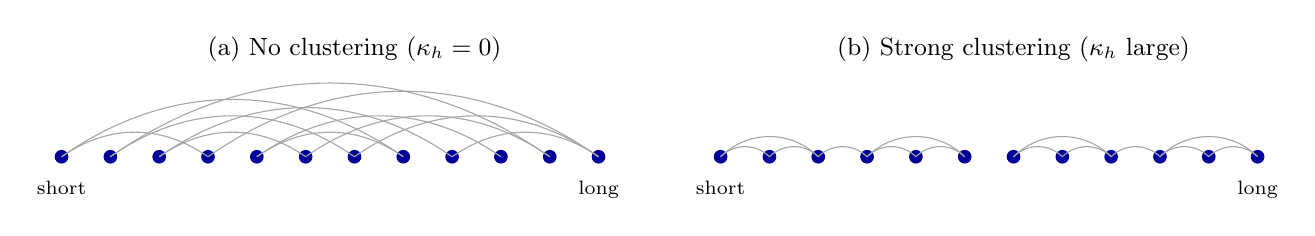
\begin{tikzpicture}[scale=0.62,>=stealth]
% left panel: no clustering
\begin{scope}
\node at (6,2.2) {\small (a) No clustering ($\kappa_h=0$)};
\foreach \i in {0,...,11} {\fill[blue!60!black] (\i,0) circle (0.14);}
\foreach \a/\b in {0/7,1/10,2/5,3/11,4/9,6/11,0/3,2/8,5/10,1/6,4/7,8/11} {\draw[gray!70] (\a,0) to[bend left=35] (\b,0);}
\node[below] at (0,-0.3) {\scriptsize short};\node[below] at (11,-0.3) {\scriptsize long};
\end{scope}
\begin{scope}[xshift=13.5cm]
\node at (6,2.2) {\small (b) Strong clustering ($\kappa_h$ large)};
\foreach \i in {0,...,11} {\fill[blue!60!black] (\i,0) circle (0.14);}
\foreach \a/\b in {0/1,1/2,0/2,3/4,4/5,3/5,6/7,7/8,6/8,9/10,10/11,9/11,2/3,8/9} {\draw[gray!70] (\a,0) to[bend left=45] (\b,0);}
\node[below] at (0,-0.3) {\scriptsize short};\node[below] at (11,-0.3) {\scriptsize long};
\end{scope}
\end{tikzpicture}
\caption{Illustration (not simulation output). Twelve investors arranged from short to long horizon. Without clustering, links cross the horizon range. With strong clustering, links join near neighbours, producing horizon-based cliques.}
\label{fig:tikz}
\end{figure}

\subsection{Horizon adaptation}

Investors are influenced by those they deal with. Every cycle, each investor moves their horizon a fraction $\eta=0.06$ of the way toward the average horizon of their linked neighbours:
\begin{equation}
\tau_i \;\leftarrow\; (1-\eta)\,\tau_i + \eta\,\bar\tau_{\mathcal N(i)} .
\label{eq:adapt}
\end{equation}
For example, a high-frequency trader with $\tau=5$ whose only neighbour has $\tau=1000$ moves to $5+0.06\times(1000-5)\approx 65$ days. In the full network, where neighbours average a few hundred days, the typical shift is more modest (about 15 days per cycle). The economic idea is a simple form of social learning: an investor who spends time among long-horizon counterparties comes to take on their way of looking at the market. Repeated over many cycles, adaptation pulls horizons together and so reduces the diversity of horizons. We call this the \emph{echo-chamber} effect.

\subsection{Three diagnostic measures}

We summarise the state of the simulated market with three numbers.

\paragraph{Horizon diversity (Temporal Diversity Index, TDI).} How spread out are investors' horizons? We split the log-horizon scale from $\ln 1$ to $\ln 2000$ into $K=16$ equal-width bins, compute the fraction $f_k$ of investors in each bin, and take the Shannon entropy,
\begin{equation}
\mathrm{TDI} \;=\; -\sum_{k=1}^{K} f_k\,\ln f_k .
\label{eq:tdi}
\end{equation}
Entropy is a standard measure of spread. If everyone sits in a single bin, TDI is zero. If investors are spread evenly over all bins, TDI is at its maximum. In the simulation the full range is available, so the largest possible value is $\ln 16\approx 2.77$. In the real-data analysis of Section~\ref{sec:data}, horizons are limited to at least 5 days, so the three lowest bins are always empty and the largest possible value is $\ln 13\approx 2.565$.

\begin{example}[Toy calculation of horizon diversity]
Suppose, to keep arithmetic small, that we use only five bins and that 20\%, 30\%, 30\%, 10\% and 10\% of investors fall in them. Then
\[
\mathrm{TDI} = -\big[0.2\ln 0.2 + 2\times 0.3\ln 0.3 + 2\times 0.1\ln 0.1\big]
= 0.322 + 0.722 + 0.461 = 1.505 .
\]
The maximum possible with five bins is $\ln 5 = 1.609$ (an even split), so this market is fairly diverse. If everyone were in one bin the value would be $0$.
\end{example}

\paragraph{Belief fragmentation (Temporal Market Fragmentation Index, TMFI).} Do investors in different horizon groups hold different beliefs about the price? We sort investors into four groups by horizon (quartiles of $\ln(\tau+1)$). Each investor forms a noisy view of the price, $\hat p_i = p\,(1+\sigma_{\mathrm{obs}}\xi_i)$ with $\sigma_{\mathrm{obs}}=0.008$ and $\xi_i$ random. We average these views within each group, and TMFI is the standard deviation of the four group averages divided by their mean:
\begin{equation}
\mathrm{TMFI}(t) \;=\; \frac{\mathrm{std}\big(\{\bar p^{(c)}(t)\}_{c=1}^{4}\big)}{\mathrm{mean}\big(\{\bar p^{(c)}(t)\}_{c=1}^{4}\big)} .
\label{eq:tmfi}
\end{equation}
Before averaging, each investor's view is blended with those of their network neighbours, with a weight that rises with the network's overall connectedness (measured by its Fiedler value, $\lambda_2$, which is a standard measure of how well connected a network is). A high TMFI means groups disagree about the price. A low TMFI means beliefs are aligned.

\paragraph{Temporal liquidity (TL).} How smoothly does price information move across horizons? We define
\begin{equation}
\mathrm{TL}(t)\;=\;\frac{1}{\sigma_r(t)\,|\mathrm{ACF}_1(t)|},
\label{eq:tl}
\end{equation}
where $\sigma_r$ is the volatility of returns and $\mathrm{ACF}_1$ is the first-order autocorrelation of returns (how strongly one period's return predicts the next). The idea is that a liquid market has both low volatility and little predictable pattern in returns. We will see in Section~\ref{sec:tl} that because volatility sits inside this measure, any comparison of TL with a volatility index is partly mechanical.

\subsection{A note on stability}

A natural worry for any simulation is whether prices simply blow up. A standard linear analysis gives a sufficient condition for stability in terms of the network: $\lambda_2>\bar\beta/\bar\alpha$. In our calibration $\bar\beta/\bar\alpha = 0.667$ while the simulated Fiedler value is about $0.655$, so the condition fails in 27 of 30 runs. This does \emph{not} mean prices explode; the condition is sufficient, not necessary. In the simulation prices stay bounded because the value-investing term in Eq.~\eqref{eq:demand} acts as a nonlinear restoring force that the linear analysis does not capture. We therefore treat the Fiedler value as a diagnostic of network connectivity, not as the governing stability criterion.

One further check concerns the simplest disturbance, a uniform shift in the price. A fractional price shift $\delta$ changes every investor's trend signal by $\delta$, and so changes next period's price by $\lambda n\bar\beta\,\delta$. Relative to the price level of 100, the one-step gain is $\lambda n \bar\beta/100 = 0.008\times 80\times 0.20/100\approx 1.3\times 10^{-3}$, far below one. A shock of this kind therefore dies out by a factor of about a thousand each period, so this mode is not a concern.

\section{Simulation Design and Results}
\label{sec:simulation}

\subsection{How the simulations were run}

Each simulation run lasts $T=500$ trading periods with $n=80$ investors, after a burn-in of 500 periods whose results are discarded so that prices settle. Because the simulation uses random numbers, a single run is only one possible outcome, so we repeat each experiment with 30 different random seeds and report averages. The main experiment sweeps the clustering strength $\kappa_h$ from 0 to 6 in 25 steps and reports results at $\kappa_h\in\{0,0.5,1,2,3,6\}$.

The fixed parameters are: price impact $\lambda=0.008$; value-investing weight $\bar\alpha=0.30$; trend weight $\bar\beta=0.20$; base noise $\sigma_0=1.0$; observation noise $\sigma_{\mathrm{obs}}=0.008$; friction coefficient $\gamma=0.20$; adaptation rate $\eta=0.06$; fundamental volatility $0.010$. To compare two settings fairly, we use a \emph{paired} design: the run at $\kappa_h=0$ and the run at $\kappa_h=6$ with the same seed share the same randomness except for the clustering strength.

\subsection{Result 1: clustering lowers volatility}
\label{sec:res1}

Raising $\kappa_h$ from 0 to 6 changes how the network is structured. A measure called \emph{assortativity} (the correlation between an investor's horizon and the average horizon of their neighbours) rises from $-0.02$, essentially random, to $0.953$, almost perfectly like-with-like.

Over 30 paired runs, the volatility of simulated returns falls by a factor of $1.310$ (paired $t=5.57$, $p=5.2\times10^{-6}$). We re-verified this with a separate 30-seed replication that gave $1.3104$ and a paired $t$ of $5.569$.

The mechanism is the friction channel of Eq.~\eqref{eq:sigeff}: clustering shrinks each investor's average distance to their counterparties, which lowers their noise and thus the total demand noise that moves the price. When we switch the friction off by setting $\gamma=0$, the gap narrows substantially, confirming that this channel is the main driver (though not necessarily the only one). The effect is moderate rather than dramatic because the model keeps four distinct investor types at every $\kappa_h$; complete homogeneity would remove friction altogether and produce a larger reduction.

\begin{figure}[htbp]
\centering
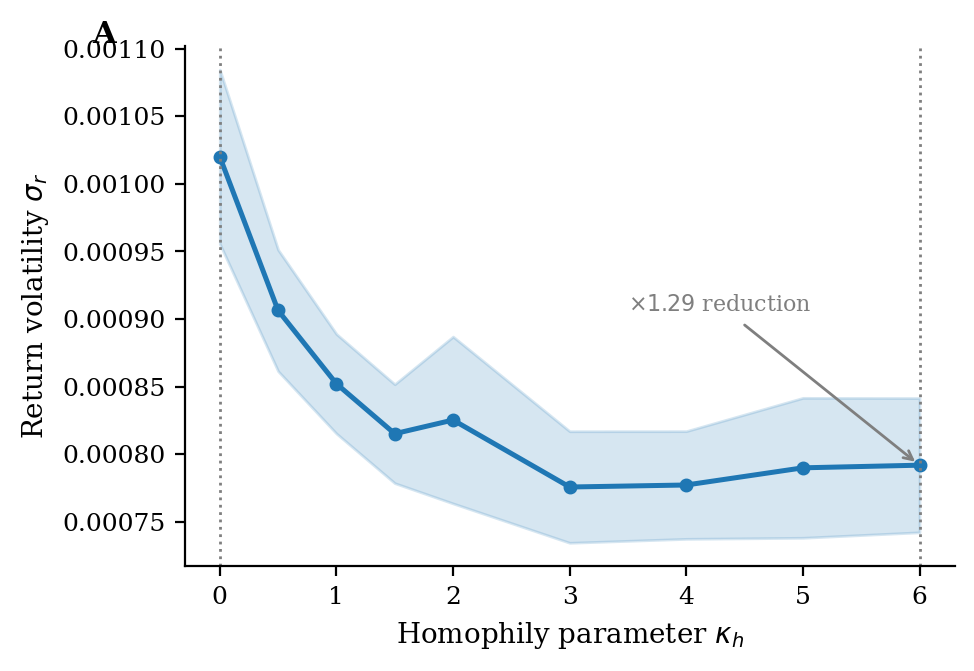
\includegraphics[width=0.78\linewidth]{fig2a}\\[4pt]
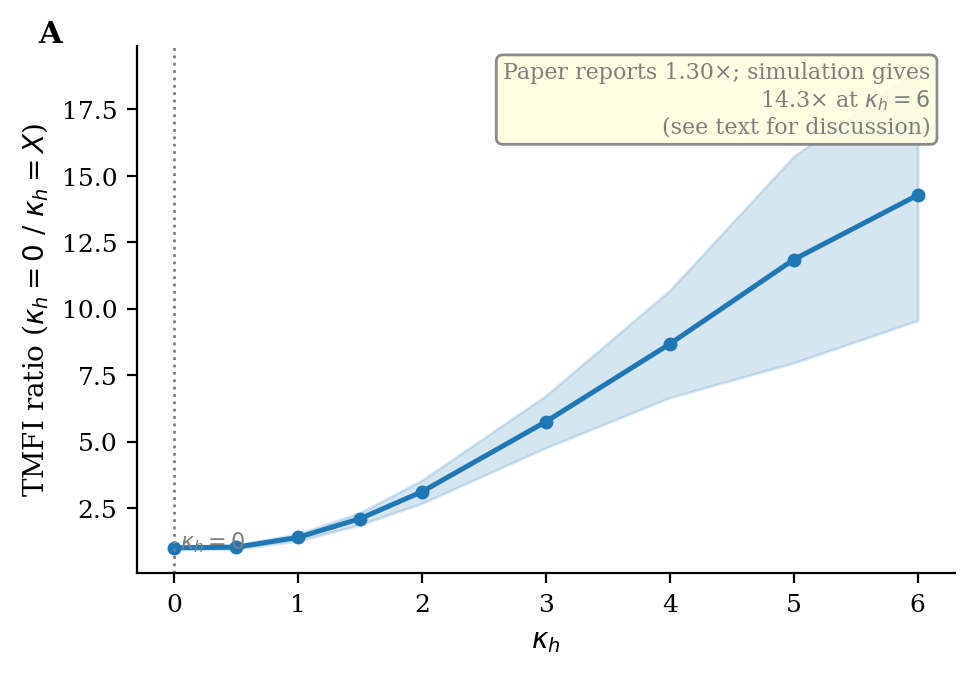
\includegraphics[width=0.78\linewidth]{fig5}
\caption{Top: simulated return volatility against clustering strength (mean and spread across 30 runs); volatility falls $1.310\times$ from $\kappa_h=0$ to $\kappa_h=6$. Bottom: belief fragmentation ratio against clustering strength; it falls $14.25\times$ by $\kappa_h=6$.}
\label{fig:vol_tmfi}
\end{figure}

\subsection{Result 2: belief fragmentation nearly disappears}

Belief fragmentation (TMFI) falls by a factor of $14.25$ from $\kappa_h=0$ to $\kappa_h=6$ (average $4.4\times10^{-4}$ falling to $3.1\times10^{-5}$; the 30-seed replication gave $14.247$). It falls much more than volatility does, for a structural reason. At $\kappa_h=0$ the network is well connected, so each investor's view is blended heavily with that of a random mix of other investors, which inflates the spread between the four horizon groups. At high $\kappa_h$, investors inside a group blend mainly with their own group and so their views converge; at the same time the global price level in the denominator is unchanged. The result is that clustering nearly eliminates disagreement \emph{between} horizon groups while only modestly lowering overall volatility. A caveat is that this ratio is a 30-seed average with considerable run-to-run variation, so it should be treated as indicative of magnitude, not a precise constant.

\subsection{Result 3: horizons drift together}
\label{sec:res3}

When adaptation is switched on (Eq.~\eqref{eq:adapt}), horizon diversity falls at every clustering strength tested. Over ten adaptation cycles the change in diversity is $-0.740$ ($\pm0.052$) at $\kappa_h=0.5$, $-0.295$ ($\pm0.061$) at $\kappa_h=3$, and $-0.306$ ($\pm0.063$) at $\kappa_h=6$ (Figure~\ref{fig:deltaTDI}). The compression is strongest when clustering is \emph{weakest}. The reason is that with weak clustering, investors are still linked to many investors with very different horizons, so the pull toward neighbours' average horizon is large; with strong clustering, neighbours already have similar horizons, so there is little to adapt toward. This is consistent in spirit with \citet{golub2012}: homophily slows convergence. The practical conclusion is that even weak clustering is enough to erode diversity, so the erosion is not confined to extreme settings.

\begin{figure}[htbp]
\centering
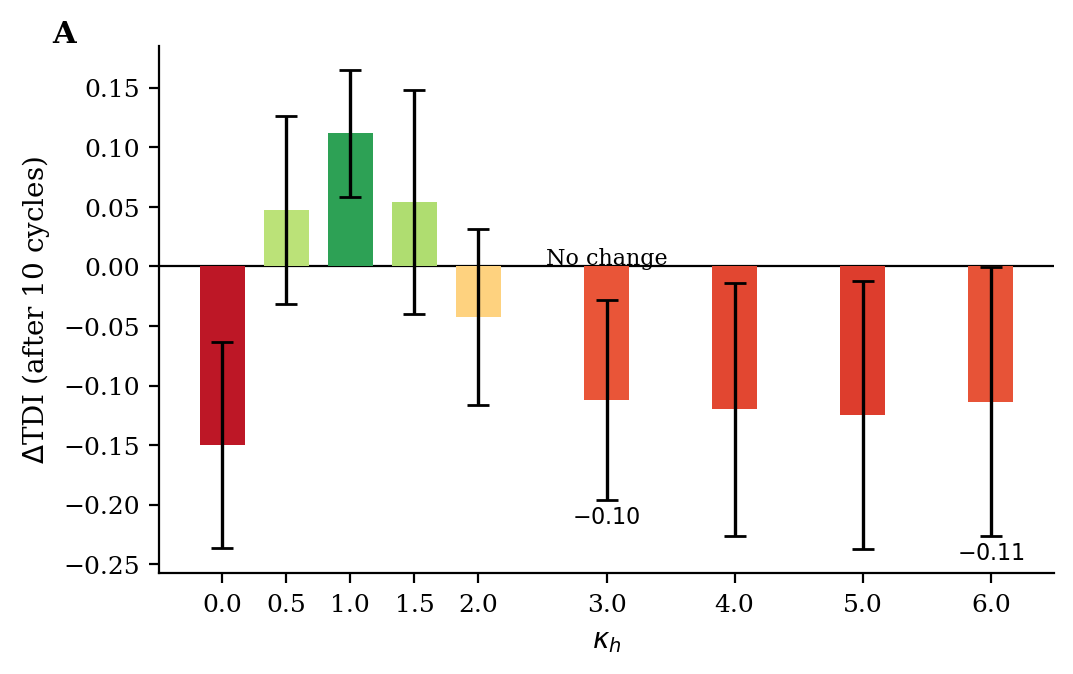
\includegraphics[width=0.78\linewidth]{fig6a}
\caption{Change in horizon diversity over ten adaptation cycles at three clustering strengths (30-run mean and spread): $-0.740$, $-0.295$ and $-0.306$ at $\kappa_h=0.5,3,6$. Every setting shows compression.}
\label{fig:deltaTDI}
\end{figure}

Together, Results 1 and 3 give the dual-channel picture that motivates the project: in the short run, clustering \emph{stabilises} (lower volatility), while over time adaptation \emph{erodes} the diversity that the Fractal Market Hypothesis regards as the foundation of stability. Whether that erosion makes markets more fragile is the part of the story that the model does \emph{not} itself deliver, as Section~\ref{sec:tension} explains.

\subsection{Result 4: temporal liquidity}

We also swept the clustering strength and recorded temporal liquidity. Mean TL appears to peak at a moderate $\kappa_h$ near 3 (Figure~\ref{fig:TLsweep}), which we initially described as a ``Goldilocks'' zone of connectivity. We now treat this cautiously: the run-to-run spread is enormous (the shaded band in the figure spans from near zero to more than five times the mean at the peak), because TL divides by a quantity that can be very small. The apparent peak is therefore not statistically distinguishable from the surrounding values, and we do not rely on it.

\begin{figure}[htbp]
\centering
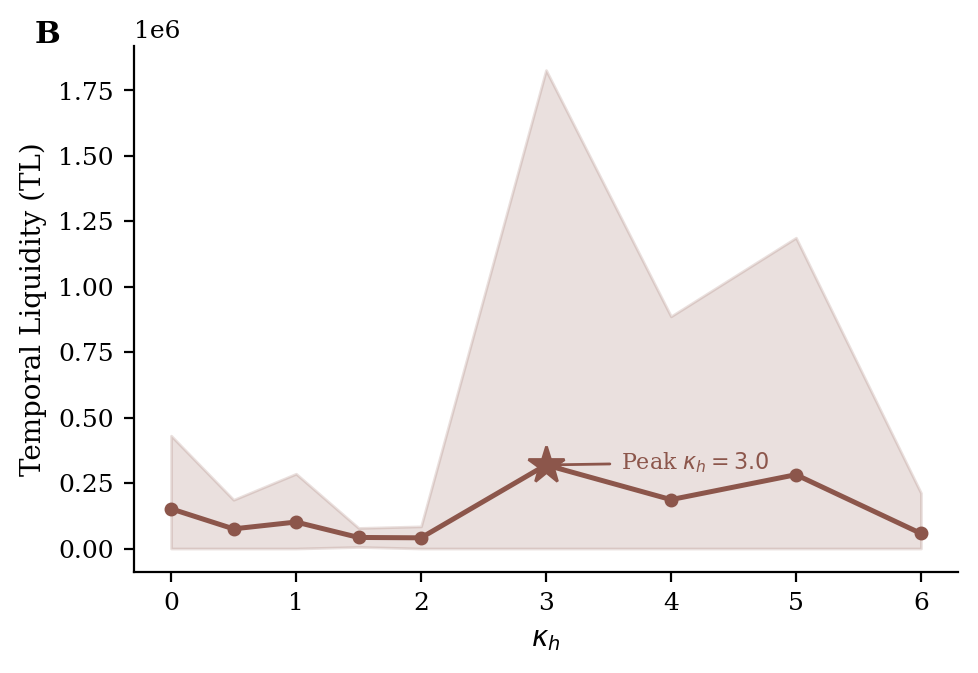
\includegraphics[width=0.7\linewidth]{fig6b}
\caption{Simulated temporal liquidity against clustering strength (mean and spread over 30 runs). The mean peaks near $\kappa_h=3$ but the spread is very large, so the peak is not statistically reliable.}
\label{fig:TLsweep}
\end{figure}

\subsection{Result 5: market composition matters (asset-class sweep)}
\label{sec:asset}

Real markets differ in who trades them. To see whether the mechanism depends on the mix of horizons, we repeated the clustering sweep with three different investor mixes, using 10 seeds at each of 25 clustering strengths: a \emph{bond market} dominated by long-horizon investors (45\% mutual-fund type and 40\% pension-fund type), the \emph{equity baseline}, and a \emph{currency and derivatives market} dominated by short-horizon investors (40\% high-frequency type and 35\% hedge-fund type).

\begin{itemize}[leftmargin=*]
\item In the \textbf{bond-like} mix, clustering raises temporal liquidity by a factor of $1.24$ (paired $t=-2.16$, $p=0.039$), and volatility falls by a factor of $1.17$ (marginal, $p=0.082$).
\item In the \textbf{currency-like} mix, all three measures are essentially flat across the whole range (all $p>0.90$): when everyone is already short-horizon, extra clustering changes little.
\item The \textbf{equity baseline} lies between the two, with no measure reaching significance ($p>0.37$).
\end{itemize}

These are simulation results, so they show that the model's effect depends on market composition, not that real bond and currency markets behave this way. They do suggest a testable implication: the mechanism should matter most in long-horizon-dominated markets.

\begin{figure}[htbp]
\centering
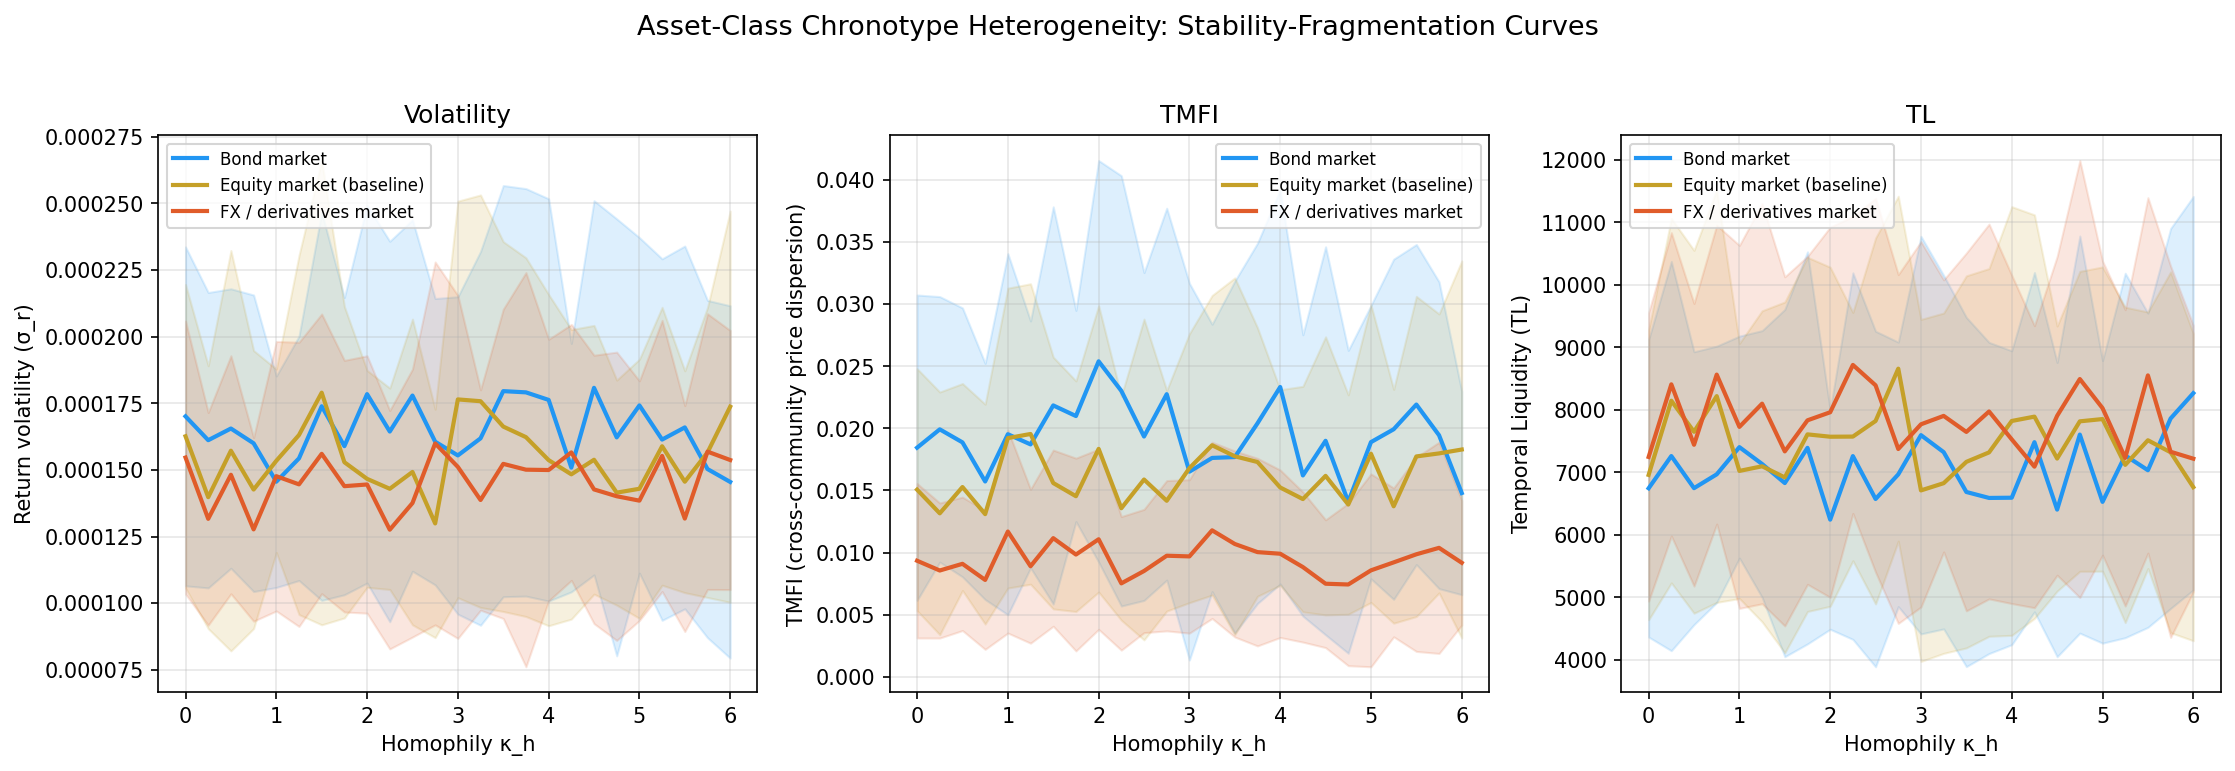
\includegraphics[width=\linewidth]{asset_class_comparison}
\caption{Simulated asset-class comparison. Panels show volatility (left), belief fragmentation (centre) and temporal liquidity (right) against clustering strength for a bond-like mix (blue), equity baseline (gold) and currency-like mix (orange). Bands are one standard deviation across runs.}
\label{fig:assetclass}
\end{figure}

\subsection{Robustness of the simulation results}

We repeated the main experiment with larger markets. At $n=160$ and $n=320$ investors, volatility still falls ($1.30\times$ and $1.34\times$ respectively, both $p<0.01$), and the Fiedler values are $0.629$ and $0.617$ at $\kappa_h=0$. Average horizon diversity rises only slightly with market size ($2.43$, $2.44$, $2.46$ for $n=80,160,320$), as expected when more investors are drawn from the same distributions. The qualitative conclusions do not change.

\subsection{A check on horizon concentration (and a correction)}
\label{sec:conc_sim}

A further question is what happens to volatility when the distribution of horizons itself is made narrower, so that investors are more alike regardless of the network. We narrow each investor type's log-normal spread by dividing its $\sigma$ by a ``compression'' factor, from $0.5$ (wider than baseline) to $3$ (much narrower). The details and a significant correction to an earlier claim are in Section~\ref{sec:tension}.

\section{Data and How We Measure Investor Horizons}
\label{sec:data}

The model is only useful if its ideas can be connected to the real world. The hardest part is that an investor's trading horizon is not recorded anywhere. We have to infer it from what investors disclose. This section explains the data and the inference step by step.

\subsection{Quarterly holdings reports (Form 13F)}

In the United States, every institutional investment manager that controls more than \$100 million in qualifying assets must file a quarterly report with the SEC, called Form 13F, listing the stocks it holds at quarter end. Each row of the report gives a security, identified by a nine-character code called a \emph{CUSIP}, and the dollar value of the position. These reports are public and free from the SEC's EDGAR system.

We use the 150 managers that file most consistently, over 52 quarters from 2013 Q1 to 2026 Q1. For our clustering analysis we use 50 usable quarters with 85 to 107 managers each. For each manager and quarter we have a list of positions. We also keep the raw reports, which additionally give the \emph{number of shares} held, because share counts (not dollar values) turn out to matter in Section~\ref{sec:drift}.

\begin{caution}[Limits of this data]
The reports show only long stock positions at quarter end. They omit short positions, many derivatives, and anything done between quarter ends. A manager that buys and sells the same stock within a quarter leaves no trace. So the horizons we infer are \emph{lower bounds on activity}, and the sample leans toward slower-moving institutions (mutual funds, pensions, insurers, endowments). Very fast traders are largely absent.
\end{caution}

\subsection{From holdings to a trading horizon}

For each manager, we compare their holdings in two consecutive quarters. Let $w_{i,s}$ denote the weight (fraction of portfolio value) manager $i$ puts on security $s$. \emph{Turnover} is the share of the portfolio that changed:
\begin{equation}
\theta_i \;=\; \tfrac12\sum_{s}\big|w_{i,s}^{\text{now}}-w_{i,s}^{\text{before}}\big| .
\label{eq:turnover}
\end{equation}
If nothing changed, $\theta_i=0$. If the manager sold everything and bought an entirely different set of stocks, $\theta_i=1$. We then convert turnover to a trading horizon in trading days:
\begin{equation}
\tau_i \;=\; \frac{63}{\theta_i}, \qquad\text{limited to the range } 5\le \tau_i\le 2000 .
\label{eq:tau}
\end{equation}
The number 63 is roughly the number of trading days in a quarter. A manager who completely turns over their portfolio each quarter ($\theta=1$) has a horizon of about one quarter (63 days). A manager who changes 10\% of the portfolio per quarter ($\theta=0.1$) has a horizon of about 630 days. We ignore managers with turnover below 0.1\% (inactive filers, which would produce absurdly long horizons).

\begin{example}[Three real managers in one quarter]
Table~\ref{tab:example} shows three managers from the 2019 Q2 data, chosen to be a fast, a typical and a slow trader. We label them A, B, C and do not identify them.
\end{example}

\begin{table}[htbp]
\centering
\caption{Three real managers in 2019 Q2. Turnover is from changes in portfolio weights.}
\label{tab:example}
\begin{tabular}{lrrrr}
\toprule
Manager & Positions held & Turnover vs.\ last quarter & Trading horizon (days) & Largest single holding\\
\midrule
A (fast) & 580 & 52.1\% & 121 & 18.1\%\\
B (typical) & 2{,}651 & 11.5\% & 548 & 2.6\%\\
C (slow) & 223 & 4.2\% & 1{,}511 & 7.1\%\\
\bottomrule
\end{tabular}
\end{table}

\subsection{From many horizons to one diversity number}

To summarise a quarter we gather the horizons of all managers with valid data, sort them into the same 16 log-scale bins used in the model, and compute the entropy of Eq.~\eqref{eq:tdi}. The result is a single number per quarter, \emph{horizon diversity}. We require at least 50 reporting managers in a quarter. This yields 45 quarters, 2013 Q3 to 2024 Q3. Horizon diversity in this sample (our original series) averages $1.86$ and ranges from $1.02$ (2022 Q4) to $1.99$ (2019 Q2).

\subsection{Market volatility indexes}

\textbf{VIX} is a published index, calculated by the Chicago Board Options Exchange from prices of options on the S\&P~500, that measures the volatility investors \emph{expect} over the next 30 days. It is widely called the market's fear gauge. We average its daily values within each quarter.

\textbf{MOVE} is the Merrill Lynch (now ICE Bank of America) Option Volatility Estimate, the analogous published index for US Treasury bonds, computed from prices of options on Treasuries. We did not create either index. (In an earlier meeting one of us described the MOVE index as something we built; that was incorrect.) We download monthly values and average them by quarter.

\subsection{Other data}

\begin{itemize}[leftmargin=*]
\item \textbf{Bond fund holdings.} Mutual funds file a different quarterly report, Form N-PORT, listing every holding including the par amount, market value and maturity date. We use it for the bond analysis (Section~\ref{sec:bonds}).
\item \textbf{Stock prices.} Daily adjusted closing prices from Yahoo Finance for individual stocks, matched to the holdings by converting CUSIPs to ticker symbols using OpenFIGI, a free public identifier service.
\item \textbf{Economic policy uncertainty.} A published index of newspaper-based policy uncertainty \citep{baker2016}, used as a control variable.
\end{itemize}

\subsection{Checking the data}

Several simple checks matter for results to be trustworthy. We keep only positions with positive value (and positive share counts when we use shares), so that no logarithm of zero or division by zero can arise. We drop managers with turnover below 0.1\%. We cap horizons at 5 and 2{,}000 days. We exclude quarters with fewer than 50 reporting managers from the diversity series and require at least 8 managers with valid horizons for the clustering score. For the stock-level work we require at least 10 owners per stock and at least 50 trading days of prices in a quarter. Appendix~\ref{app:checks} gives the full list.

\section{Empirical Findings}
\label{sec:findings}

This section reports what we found when we confronted the model with data. Each subsection states the question, describes the data and method, gives the result, and says what it does and does not show.

\subsection{Do investors with similar horizons hold similar portfolios?}
\label{sec:kappa}

\paragraph{Why this matters.} The central assumption of the model is that like trades with like. If real investors with similar horizons did not hold similar things, the clustering mechanism would have no counterpart in reality. This is the most direct empirical test of the model's foundation.

\paragraph{How we measure it.} In a given quarter, take every pair of managers $(i,j)$. For each pair compute two numbers.
\begin{enumerate}[leftmargin=*]
\item \emph{Portfolio similarity}: the cosine similarity of their portfolio weight vectors. Think of each portfolio as a list of weights over all securities. Cosine similarity is $1$ if two portfolios hold identical proportions of identical securities, and $0$ if they have no security in common.
\item \emph{Horizon closeness}: $\exp\!\big(-|\ln(\tau_i+1)-\ln(\tau_j+1)|\big)$. This equals $1$ for identical horizons and falls toward $0$ as horizons diverge. It is the same kernel the model uses to form links (Eq.~\eqref{eq:network} with $\kappa_h=1$).
\end{enumerate}
The \emph{horizon clustering score} $\hat\kappa_h$ for the quarter is the correlation, across all pairs, between these two numbers. A positive score means pairs with closer horizons hold more similar portfolios.

\begin{example}[Three pairs]
Using managers A, B, C from Table~\ref{tab:example}:
\begin{center}
\begin{tabular}{lrrr}
\toprule
Pair & Securities both hold & Portfolio similarity & Horizon closeness\\
\midrule
A and B & 346 & 0.079 & 0.222\\
A and C & 43 & 0.001 & 0.081\\
B and C & 195 & 0.132 & 0.363\\
\bottomrule
\end{tabular}
\end{center}
The pair with the closest horizons (B and C) also has the most similar portfolios, and the pair with the most distant horizons (A and C) has almost no overlap. Repeating this for every pair, roughly 3{,}600 to 5{,}700 pairs per quarter, gives the score.
\end{example}

\paragraph{Result.} The score is positive in all 50 quarters. Its average is $+0.158$ (standard deviation $0.043$ across quarters), with a smallest value of $0.051$ (Figure~\ref{fig:kappa}). Real investors with similar horizons do hold more similar portfolios. The effect is modest in size but remarkably consistent.

\begin{figure}[htbp]
\centering
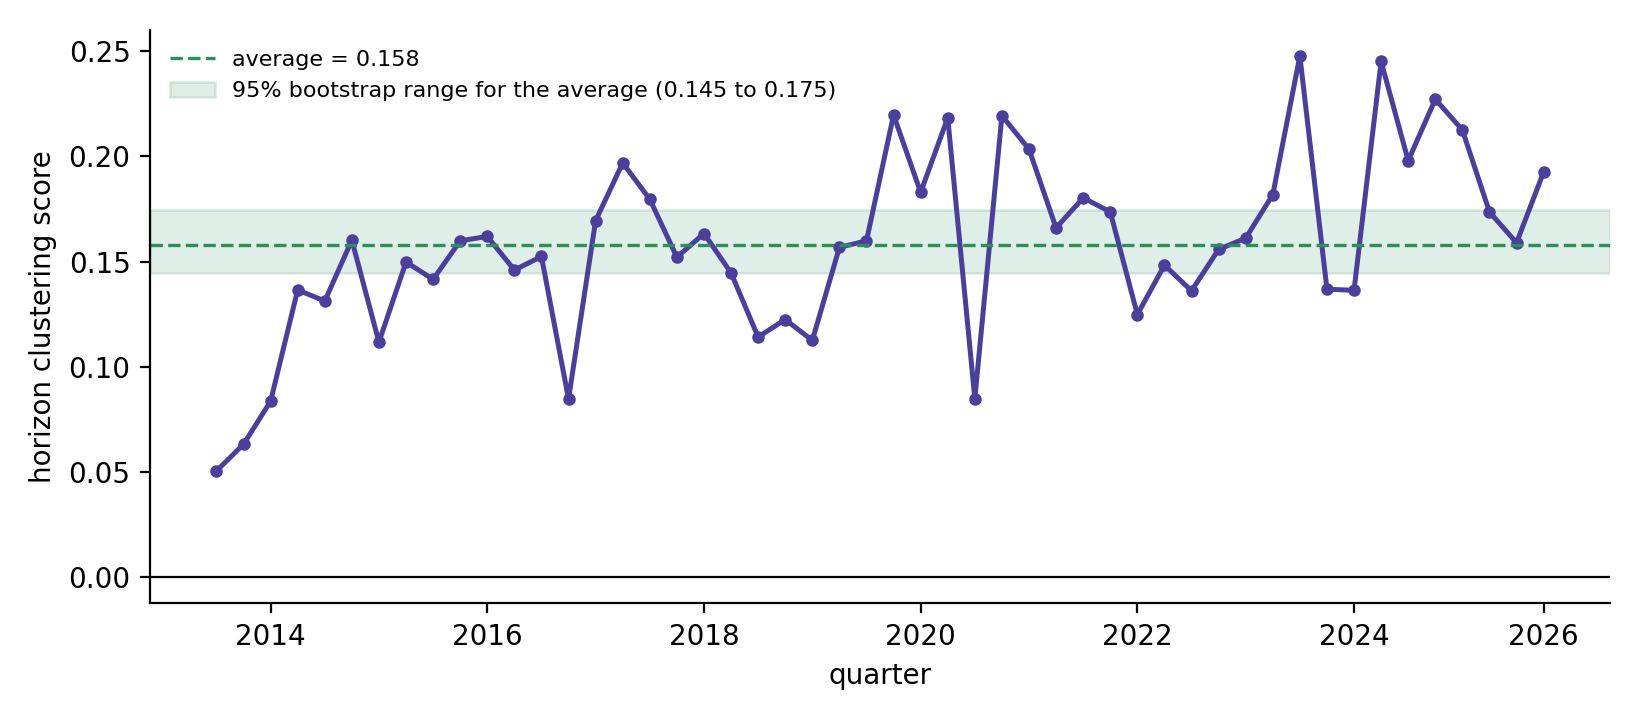
\includegraphics[width=0.85\linewidth]{kappa_series}
\caption{The horizon clustering score for each quarter, 2013 Q3 to 2026 Q1. The score is positive throughout. The shaded band is a 95\% range for the average obtained by resampling blocks of four quarters.}
\label{fig:kappa}
\end{figure}

\paragraph{How sure are we? Correcting for time dependence.} A simple test of whether the average differs from zero treats the 50 quarterly scores as independent, giving a $t$-statistic of $25.7$. But quarters are not independent: portfolios change slowly, so one quarter's score resembles the previous one. The correlation between one quarter's score and the next is $0.35$. A standard test confirms the pattern (the Ljung--Box test rejects ``no pattern'' at $p=0.012$ with one lag and $p=0.023$ with four, but not with eight lags, $p=0.10$).

The standard fix is the \emph{Newey--West correction}, which widens the uncertainty estimate to allow for each quarter resembling those nearby. It requires choosing a number of \emph{lags}, meaning how many neighbouring quarters are allowed to be related. A reviewer's natural question is how many lags are needed. Two standard formulas (Schwert's and Newey and West's 1994 rule) both give 3 lags. A third rule based on the series' own persistence gives 4. We also report longer lags up to 8 as a deliberately conservative check. Table~\ref{tab:lags} shows the result.

\begin{table}[htbp]
\centering
\caption{Newey--West $t$-statistic for the average clustering score being zero. A $t$ above about 2 is significant.}
\label{tab:lags}
\begin{tabular}{rrr}
\toprule
Lags & Standard error & $t$-statistic\\
\midrule
0 (no correction) & 0.0061 & 25.7\\
1 & 0.0071 & 22.1\\
2 & 0.0078 & 20.2\\
3 (chosen by two rules) & 0.0083 & 19.0\\
4 (chosen by third rule) & 0.0087 & 18.2\\
6 & 0.0093 & 17.1\\
8 & 0.0097 & 16.3\\
\bottomrule
\end{tabular}
\end{table}

More lags make the correction more cautious and the $t$-statistic falls, but it stays far above any threshold at every lag count. An earlier draft of our paper stated that the corrected statistic was about $15$ and referred to an effective sample size of 17; that figure came from a rough approximation and had never been computed. The effective sample size is in fact about 24 (computed as $50\times(1-0.35)/(1+0.35)$).

Two further checks agree. A \emph{block bootstrap}, which resamples blocks of four consecutive quarters to preserve their dependence, gives a 95\% range for the average of $0.145$ to $0.175$. A \emph{permutation test} addresses a separate problem: the roughly 5{,}000 pairs within a quarter are not independent of each other, since each manager appears in many pairs. We therefore reshuffle the horizons across managers 500 times within each quarter and ask how often a shuffled score is as large as the real one. The real score beats the shuffles at the 5\% level in 48 of 50 quarters (the exceptions are 2013 Q3 and 2013 Q4, the earliest quarters, with fewer reporting managers) and at the 1\% level in 47 of 50 (the third exception is 2016 Q4). This replaces an earlier claim that the score was highly significant in \emph{every} quarter, which did not survive the permutation test.

\paragraph{What the score does not show.} The score relates horizons to \emph{holdings} at one date, not to purchases or trades, so it does not show that investors \emph{buy} the same things. It also does not by itself tell us why horizon-similar managers hold similar stocks. And its relationship with the VIX is in the predicted direction but not significant ($r=+0.14$, $p=0.33$, 50 quarters).

\subsection{Is horizon diversity related to market volatility?}
\label{sec:drift}

\subsubsection{The original result}

Our original main empirical result was that horizon diversity (Eq.~\eqref{eq:tdi}) moves opposite to the VIX. Over 45 quarters, 2013 Q3 to 2024 Q3, the correlation is $r=-0.526$ ($p=0.0002$). Diversity was lowest in the Fed-tightening quarter 2022 Q4 ($1.02$) and fell sharply in the COVID-19 quarter 2020 Q1 ($1.55$); it was highest in calm 2019 Q2 ($1.99$). Figure~\ref{fig:tdi} shows the series.

\begin{figure}[htbp]
\centering
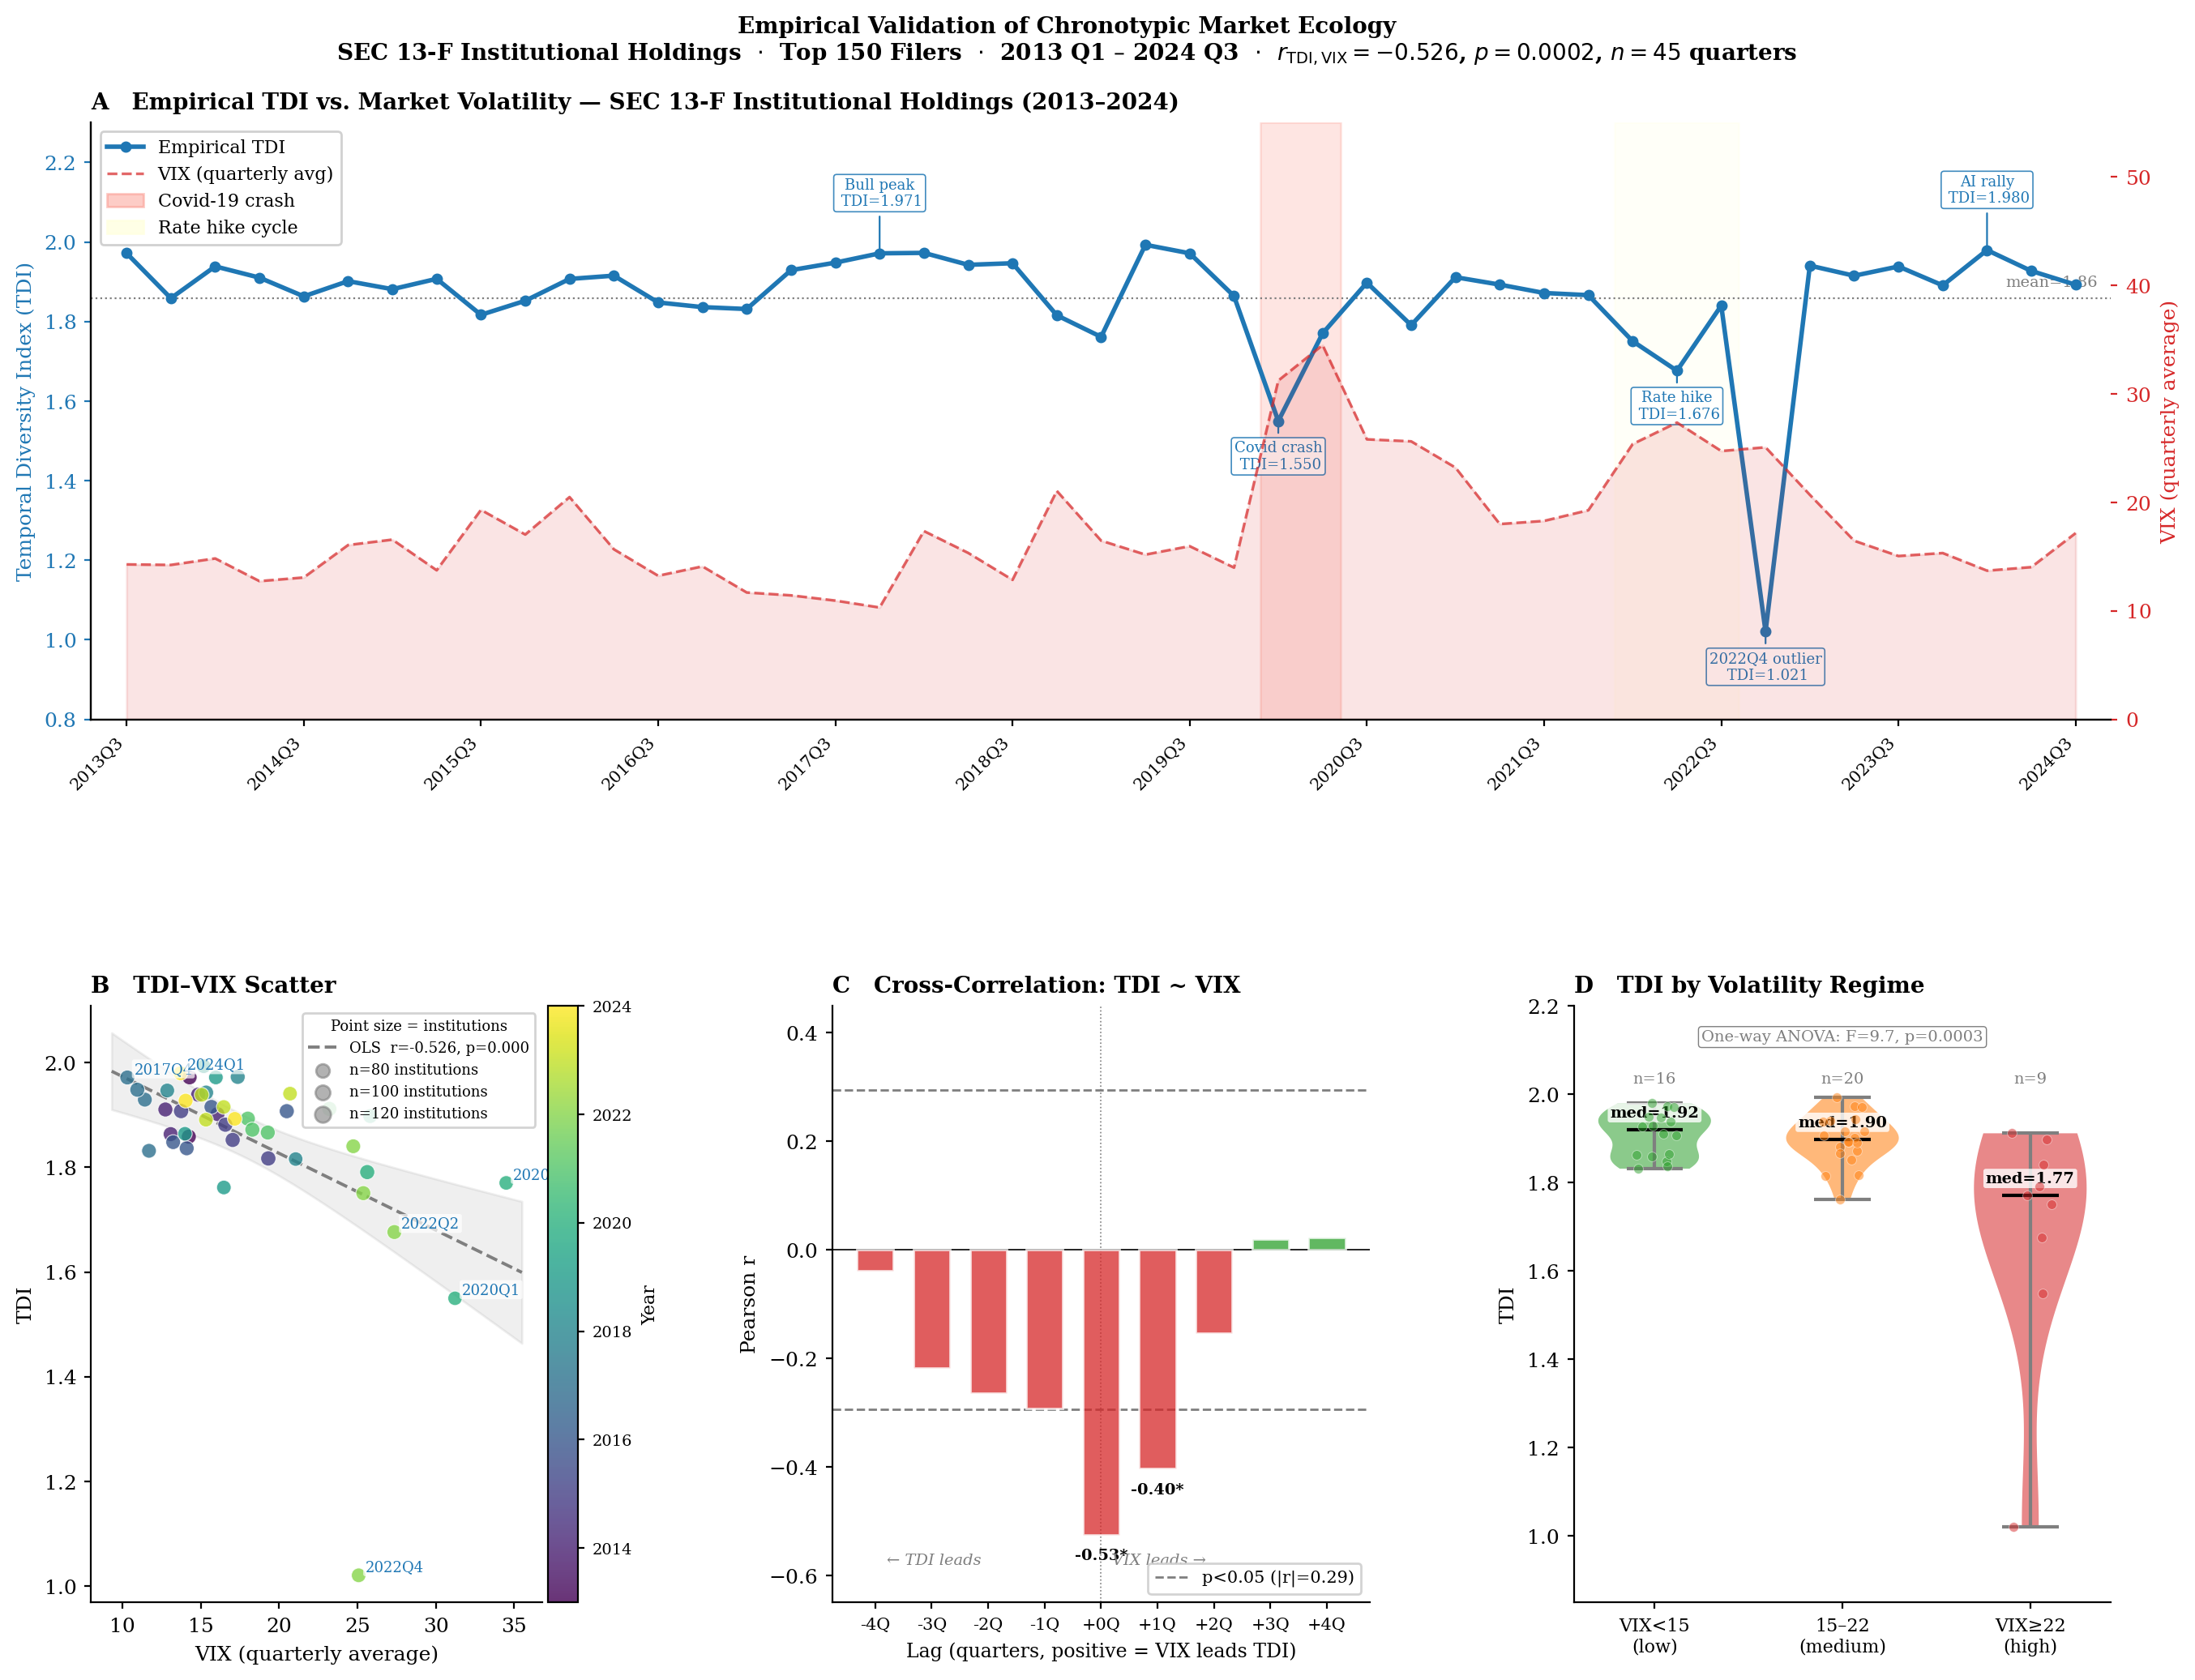
\includegraphics[width=\linewidth]{empirical_tdi_validation}
\caption{Original horizon diversity series (blue) and quarterly VIX (red dashed), 2013 Q3 to 2024 Q3.}
\label{fig:tdi}
\end{figure}

We also asked which series leads. A \emph{Granger test} asks whether last quarter's value of one series helps predict this quarter's value of another, beyond what the second series' own past predicts. It is a test of lead and lag, not proof of cause. In our original series, the VIX helps predict future diversity ($F=4.13$, $p=0.049$) but diversity does not help predict the VIX ($F=0.13$, $p=0.72$). Read naively, this says volatility compresses horizon diversity, the reverse of the direction in the model's story. A shock to diversity of one standard deviation reduces the VIX by about 1.9 points on impact in an impulse-response analysis, and an extended regression with policy-uncertainty and market-return controls gives an imprecise coefficient ($-3.80$, $p=0.18$). We reported these results while noting that the first was inconsistent with the direction the model emphasises.

\subsubsection{A problem we then found: price drift}

\begin{caution}[The central correction of this document]
Our measure of how often a manager trades turns out to be contaminated by price movements. When we remove that contamination, the link between horizon diversity and the VIX disappears.
\end{caution}

The turnover measure of Eq.~\eqref{eq:turnover} uses \emph{portfolio weights}, which are each holding's share of the portfolio's dollar value. But weights change whenever prices change, even if the manager does nothing at all.

\begin{example}[A manager who never trades]
A manager holds two stocks in equal amounts, so each has weight $50\%$. Over a quarter, stock A rises $10\%$ and stock B falls $10\%$, and the manager does nothing. The new weights are $1.10/2.00=55\%$ and $0.90/2.00=45\%$. The weight-based turnover is $\tfrac12(|0.55-0.50|+|0.45-0.50|)=5\%$, which implies a horizon of $63/0.05=1{,}260$ days. A true no-trade manager has an infinite horizon, so the measure has invented activity. In a volatile quarter, with bigger price moves, the invented turnover is bigger.
\end{example}

In volatile quarters prices move more, so weight-based turnover rises for everyone and horizons \emph{look} shorter, even with no change in behaviour. This would create a negative correlation between horizon diversity and the VIX with no behavioural content.

\paragraph{The test.} We rebuilt turnover from \emph{share counts} instead. For each security we use a single price (so that price changes cannot generate trades) and measure how many shares the manager actually bought or sold, as a fraction of the portfolio's value. We also repeat it after rebasing for stock splits, which change share counts without any trading. Everything else, including the managers, the bins and the formula, is unchanged.

Using our rebuilt data and the same VIX as the original (45 quarters), the correlation of horizon diversity with the VIX is:

\begin{table}[htbp]
\centering
\caption{Correlation of horizon diversity with the VIX under different turnover measures.}
\label{tab:drift}
\begin{tabular}{lrr}
\toprule
How turnover is measured & Correlation with VIX & 95\% range\\
\midrule
Change in portfolio weights (original method) & $-0.59$ & $-0.80$ to $-0.24$\\
Change in share counts & $-0.06$ & $-0.43$ to $+0.25$\\
Change in share counts, splits adjusted & $-0.10$ & $-0.49$ to $+0.27$\\
\bottomrule
\end{tabular}
\end{table}

The ranges come from a block bootstrap. The difference between the first two correlations is itself significant (95\% range $-0.92$ to $-0.13$). Figure~\ref{fig:drift} shows the two versions side by side. The weight-based measure tracks the VIX; the share-based measure does not.

\begin{figure}[htbp]
\centering
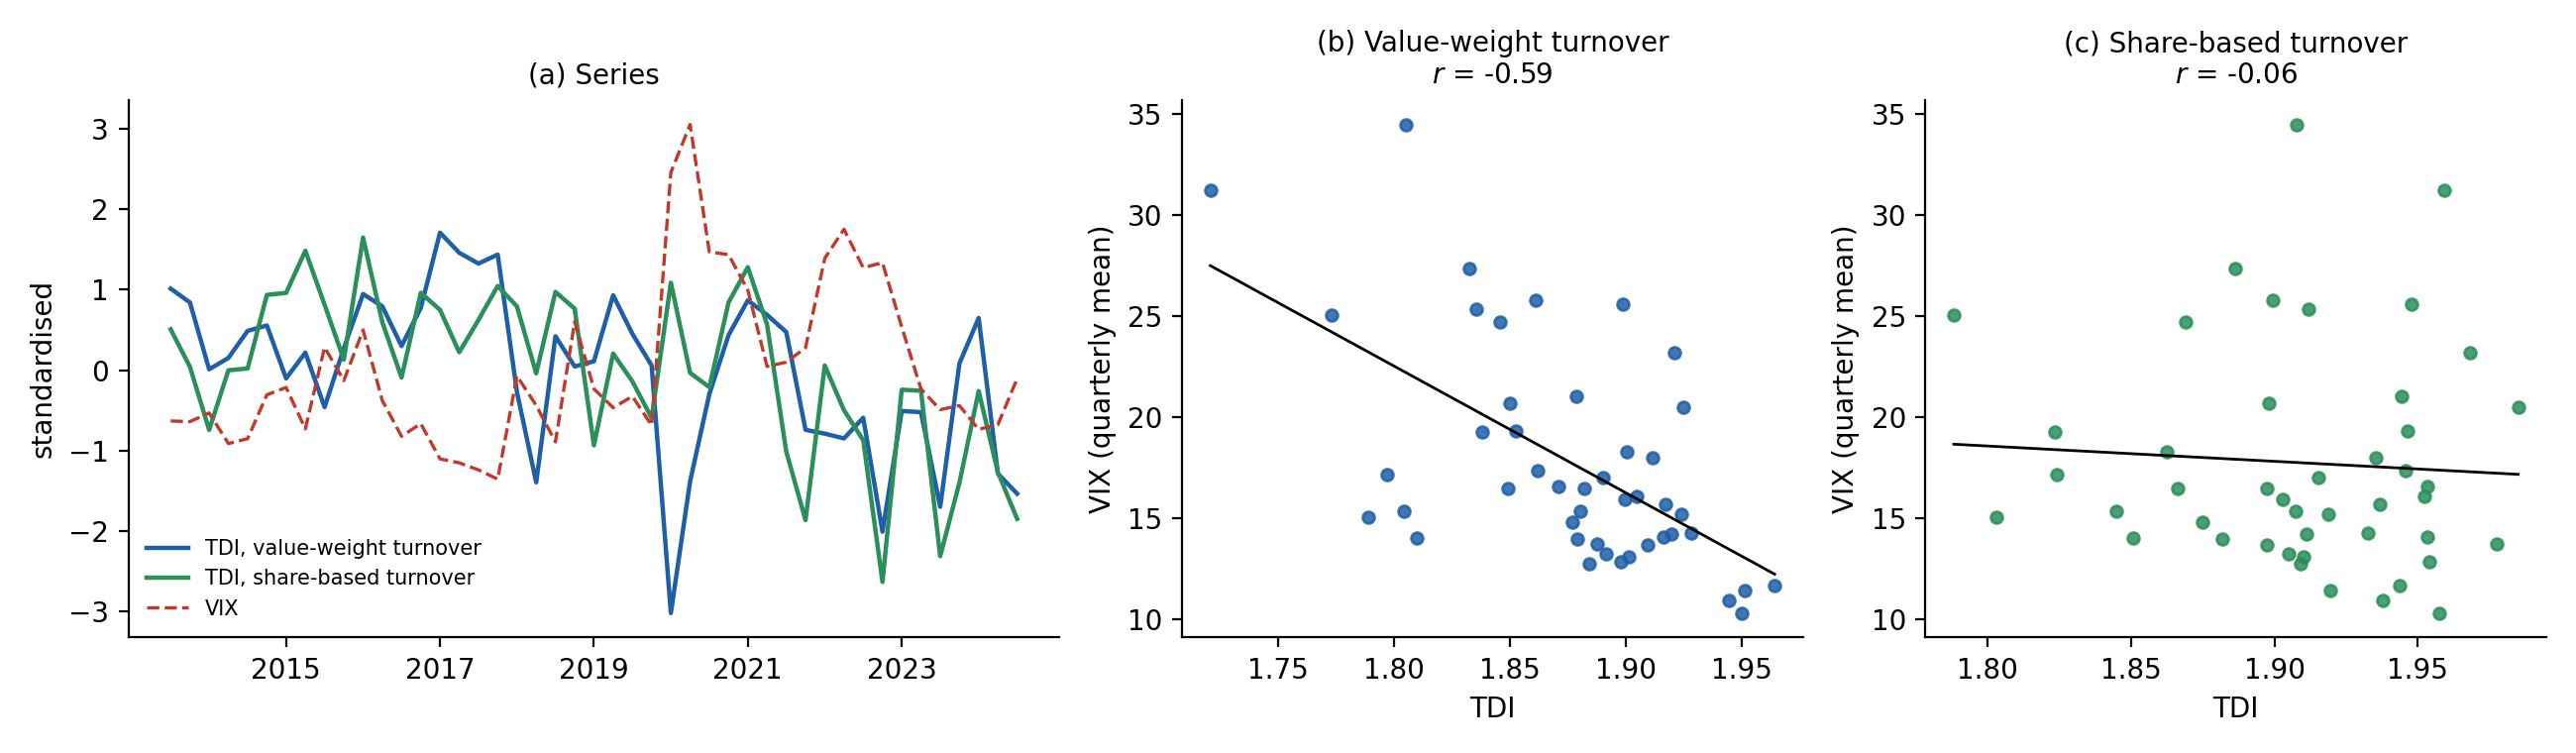
\includegraphics[width=\linewidth]{drift_check}
\caption{(a) Standardised horizon diversity built from weight-based turnover (blue) and share-based turnover (green), with the VIX (red dashed). (b) The weight-based measure falls when the VIX is high. (c) The share-based measure shows no relationship.}
\label{fig:drift}
\end{figure}

\paragraph{What this means.} Most of our original headline empirical result was a measurement effect. It should not be read as evidence that horizon diversity responds to, or influences, volatility. The Granger lead we found does not reproduce on the rebuilt series (VIX leads weight-based diversity at $p=0.73$ and share-based diversity at $p=0.21$, neither significant; with splits adjusted $p=0.08$), so we treat it as suggestive only.

\begin{caution}[A discrepancy we have not resolved]
Our rebuilt diversity series uses a somewhat different set of managers (114 to 135 per quarter versus 94 to 108 originally) and correlates only 0.50 with the original series. The largest gap is 2022 Q4, where the original series shows the lowest value in the sample ($1.02$) and the rebuilt one shows $1.77$. We have not identified the cause. For this reason, the comparison above is valid \emph{between turnover methods within the rebuilt data}, not as an exact copy of the original numbers.
\end{caution}

\subsubsection{Could there still be a real behavioural link?}

\citet{harrisraviv1993} argue that when investors disagree more, they trade more. Volatile times are times of greater disagreement, so a genuine behavioural reason for horizons to shorten when volatility rises is plausible. Our price-drift test shows that the \emph{accounting} channel explains most of what we measured. It does not rule out a real behavioural effect, only that our data cannot detect one. Separating the two would need trade-level data, or an event in which disagreement changes without price moving.

\subsection{Temporal liquidity: a result that was largely mechanical}
\label{sec:tl}

We built an empirical version of temporal liquidity from the S\&P~500 exchange-traded fund SPY. Each quarter we compute the volatility of quarterly returns over a rolling 4-quarter window and the first-order autocorrelation over a rolling 8-quarter window (using prices from 2011 so that every one of the 45 quarters is covered), and form TL by Eq.~\eqref{eq:tl}. The correlation of TL with the VIX is $-0.392$ ($p=0.008$, 45 quarters).

This looks like support for the model, but it is largely mechanical. Return volatility is \emph{inside} TL, in the denominator, so the logarithm of TL and minus the logarithm of volatility correlate at $0.90$. Realised return volatility correlates with the VIX at $0.76$, because the VIX tracks realised volatility. The other ingredient, return autocorrelation, which is the part carrying the model's mechanism, is unrelated to the VIX ($r=+0.04$, $p=0.81$). So the negative TL--VIX correlation tells us only that volatility is correlated with volatility. We do not count it as evidence for the mechanism. (An earlier draft reported this correlation on 36 quarters with an explanation about a burn-in period; the numbers are in fact from all 45 quarters, and that explanation was wrong.) TL is also uncorrelated with horizon diversity ($r=0.10$, $p=0.51$).

\subsection{Bond funds}
\label{sec:bonds}

\subsubsection{First attempt: average maturity}

Bond funds file holdings reports (Form N-PORT) that list every bond with its maturity date. For three large fund families (PIMCO, Vanguard, BlackRock), we computed each fund's \emph{weighted average maturity}, the dollar-weighted average of the remaining years to maturity, converted it to a horizon ($\text{years}\times252$ trading days), computed horizon diversity across funds each quarter, and correlated it with the MOVE index over 12 quarters, 2024 to 2026. The correlation was $-0.213$ ($p=0.51$), indistinguishable from zero.

We interpret this as an honest null result with an identifiable cause. Weighted average maturity reflects how a fund is \emph{built} (a short-term fund versus a long-term fund), set by its mandate and changing slowly, not how actively it \emph{trades}. The CME mechanism needs variation in active trading horizons, which this proxy does not capture.

\subsubsection{Second attempt: behavioural horizons by credit quality}

A reviewer suggested comparing bond funds with very different information environments, since in Treasury bonds essentially everyone has the same information whereas in high-yield (``junk'') corporate bonds some investors may know much more than others. We took seven Vanguard bond funds: short-, intermediate- and long-term Treasury; short-, intermediate- and long-term investment-grade corporate; and high-yield corporate. Each has 28 quarterly reports, giving 27 quarter-to-quarter changes.

To capture trading behaviour instead of fund design, we measure turnover from changes in the \emph{par amount} of each bond held, valued at a single price per bond so that price changes cannot generate trades, and we exclude bonds that simply matured. The behavioural horizon is then $63/\theta$ as before.

\begin{table}[htbp]
\centering
\caption{Seven Vanguard bond funds, 27 quarterly changes each. ``Link'' is the correlation across quarters, within each fund, with the MOVE index.}
\label{tab:bonds}
\small
\begin{tabular}{lrrrr}
\toprule
Fund & Average maturity (years) & Median trading horizon (days) & Link: maturity & Link: horizon\\
\midrule
Short-term Treasury & 3.75 & 146 & $-0.30$ & $+0.45$\\
Intermediate-term Treasury & 6.63 & 211 & $-0.54$ & $+0.44$\\
Long-term Treasury & 21.97 & 400 & $-0.40$ & $+0.30$\\
Short-term investment grade & 4.29 & 437 & $-0.64$ & $+0.47$\\
Intermediate-term investment grade & 8.40 & 363 & $-0.41$ & $+0.73$\\
Long-term investment grade & 22.84 & 765 & $-0.28$ & $+0.01$\\
High-yield corporate & 5.52 & 667 & $-0.31$ & $+0.36$\\
\bottomrule
\end{tabular}
\end{table}

Grouped by type, the median trading horizon is 218 days for Treasury funds, 454 days for investment-grade corporate funds and 667 days for high-yield funds. The funds with the most uncertain, dispersed information trade least often. Within each type, the behavioural horizon moves with the MOVE index with similar strength ($+0.38$ Treasury, $+0.33$ investment grade, $+0.36$ high yield): funds trade \emph{less} often when bond-market volatility is high. This is the opposite sign to the (now discounted) equity relationship in which horizons appeared to shorten when volatility rose, and it is consistent with a view that bond funds retreat in stressed periods. The average-maturity measure moves the other way (negative, as in the table), which fits the idea that maturity captures fund design and moves with the interest-rate environment rather than activity.

\begin{caution}[Interpret with care]
Each fund has only 27 observations and neighbouring quarters overlap. The pooled $p$-values within a type treat fund-quarters as independent although every fund in a given quarter shares one MOVE value, so we do not present them as formal tests. The results are descriptive.
\end{caution}

\subsection{A test on individual stocks}
\label{sec:stock}

\paragraph{Why move to stocks.} The aggregate relationship uses only 45 quarterly points, which gives little power and no way to control for other influences. Individual stocks give thousands of observations. The Fractal Market Hypothesis predicts that a stock owned by a narrow range of horizons should be more fragile than one owned by a wide mix. We can test that directly.

\paragraph{Measuring owner-horizon spread.} For a stock $s$ in a quarter, we take its owners among our panel of managers (requiring at least 10 owners). Let $w_{i,s}$ be manager $i$'s share of the panel's total dollar holding of $s$, and $\tau_i$ the manager's horizon from share-based turnover. The ownership-weighted average log horizon and spread are
\begin{equation}
\mu_s=\sum_i w_{i,s}\ln\tau_i,\qquad
\mathrm{DISP}_s=\sqrt{\sum_i w_{i,s}\,(\ln\tau_i-\mu_s)^2}.
\label{eq:disp}
\end{equation}
Low $\mathrm{DISP}_s$ means the stock's owners have similar horizons.

\paragraph{The question and the prediction.} Does low $\mathrm{DISP}_s$ in one quarter predict high volatility the next quarter? We fixed the prediction before looking at outcomes: the hypothesis predicts a \emph{negative} relationship (less spread, more volatility). The outcome is the log of the next quarter's realised volatility (standard deviation of daily returns, annualised). We also looked at the worst daily return and the skewness of returns as secondary outcomes.

\paragraph{Controls and methods.} Stocks differ in many ways, so we control for the owners' average horizon $\mu_s$ (which means we are asking about \emph{spread}, not about how short-term the owners are, which is the question of \citealt{cella2013}), the number of owners, how concentrated ownership is, the dollar amount held by our panel (a rough size proxy) and the stock's own current-quarter volatility (to guard against volatility simply persisting). All variables are standardised, so a coefficient reads as the change in next-quarter volatility, in standard deviations, per one standard deviation of owner spread.

We estimate in three ways. \emph{Fama--MacBeth} runs a separate cross-sectional regression each quarter and averages the coefficients, with the Newey--West correction on the time series of coefficients. \emph{Pooled with quarter fixed effects} compares stocks within the same quarter. \emph{Stock plus quarter fixed effects} compares each stock only with itself over time, removing anything permanent about a stock such as being large or being a blue chip; it is the most demanding test. As a falsification test (a \emph{placebo}), we randomly shuffle horizons across managers within each quarter, which should destroy any real relationship.

\paragraph{Data.} Starting from 44{,}573 distinct securities in the holdings, 2{,}449 had at least 10 owners in at least 30 quarters. After mapping to ticker symbols and keeping stocks with usable price histories, the sample is 63{,}261 stock-quarters covering 1{,}699 stocks over 48 quarters.

\begin{table}[htbp]
\centering
\caption{Effect of owner-horizon spread on next-quarter log volatility (standardised coefficients; more negative means that less spread goes with more volatility).}
\label{tab:stock}
\begin{tabular}{lrr}
\toprule
Method & Share-based horizons & Weight-based horizons\\
\midrule
Fama--MacBeth, average across quarters & $-0.046$ ($t=-6.2$) & $-0.044$ ($t=-8.0$)\\
Pooled, quarter fixed effects & $-0.017$ ($t=-4.1$) & $-0.009$ ($t=-2.3$)\\
Stock and quarter fixed effects & $-0.011$ ($t=-2.4$, $p=0.016$) & $-0.005$ ($p=0.26$)\\
Placebo (horizons shuffled) & $0.000$ ($t=0.01$) & not run\\
\bottomrule
\end{tabular}
\end{table}

\paragraph{Result.} Across stocks the relationship has the predicted sign and is statistically strong (Table~\ref{tab:stock}). But the effect shrinks as the comparison becomes more demanding. Within a single stock over time the coefficient is $-0.011$: a one-standard-deviation change in owner spread moves next-quarter volatility by about 1\% of a standard deviation. That is statistically detectable ($p=0.016$) but economically tiny, and with the weight-based horizons the within-stock effect is not significant. The placebo gives zero, as it should. The two secondary outcomes were not consistent: the worst daily return has the predicted sign in the Fama--MacBeth estimate but the opposite sign with fixed effects, and skewness shows no relationship.

\begin{caution}[Limits of the stock-level test]
(i) The price data are free data from Yahoo Finance, which \emph{drops delisted and acquired companies}, so the sample contains only survivors, which can bias volatility results. (ii) Only about 60\% of securities were matched to tickers, and current tickers can differ from historical ones. (iii) We have no true market capitalisation, so size is controlled only roughly, although the stock fixed effects remove permanent size differences. (iv) Our holdings cover 150 managers, not all institutions. The standard solution is the CRSP database, discussed in Section~\ref{sec:future}.
\end{caution}

\section{Where the Model and the Data Disagree}
\label{sec:tension}

\subsection{What the data say}

The stock-level test of Section~\ref{sec:stock} found that stocks whose owners have \emph{similar} horizons are slightly \emph{more} volatile the next quarter. That is the pattern the Fractal Market Hypothesis predicts: concentrated horizons are fragile.

\subsection{What the model says}

An earlier version of our paper claimed that the model produced the same pattern, that narrowing the distribution of horizons both lowers horizon diversity and \emph{raises} volatility. We have now tested this properly and found that the claim was unsupported.

The earlier check built a narrower horizon distribution but then called the simulation routine, which drew its own horizons internally, so the narrower horizons never reached the simulated market. Whatever relationship appeared came from random variation between runs. We fixed this by feeding the narrower horizons into the actual simulation. We narrow each investor type's log-normal spread by dividing its $\sigma$ by a compression factor running from 0.5 (wider than baseline) to 3 (much narrower), and run 25 simulations at each factor for two clustering strengths.

\begin{table}[htbp]
\centering
\caption{Simulated volatility when the horizon distribution is compressed. Horizon diversity is computed with the fixed 16-bin definition (Eq.~\eqref{eq:tdi}). Volatility is multiplied by 1{,}000 for readability. 25 runs per cell.}
\label{tab:conc}
\begin{tabular}{lrrrrr}
\toprule
Compression factor & 0.5 & 1.0 & 1.5 & 2.0 & 3.0\\
\midrule
Horizon diversity & 2.52 & 2.44 & 2.29 & 2.17 & 2.01\\
Volatility, clustering strength 0.5 & 0.95 & 0.94 & 0.95 & 0.92 & 0.84\\
Volatility, clustering strength 2.0 & 0.86 & 0.88 & 0.79 & 0.80 & 0.80\\
\bottomrule
\end{tabular}
\end{table}

At clustering strength 0.5, volatility at the strongest compression is lower than at the weakest (Welch $t=-2.72$, $p=0.009$). At strength 2.0 the difference points the same way but is not significant ($p=0.13$). Across individual runs, horizon diversity and volatility are \emph{positively} correlated ($r=+0.21$, $p=0.02$ at strength 0.5; $r=+0.17$, $p=0.06$ at strength 2.0). Figure~\ref{fig:conc} shows this.

\begin{figure}[htbp]
\centering
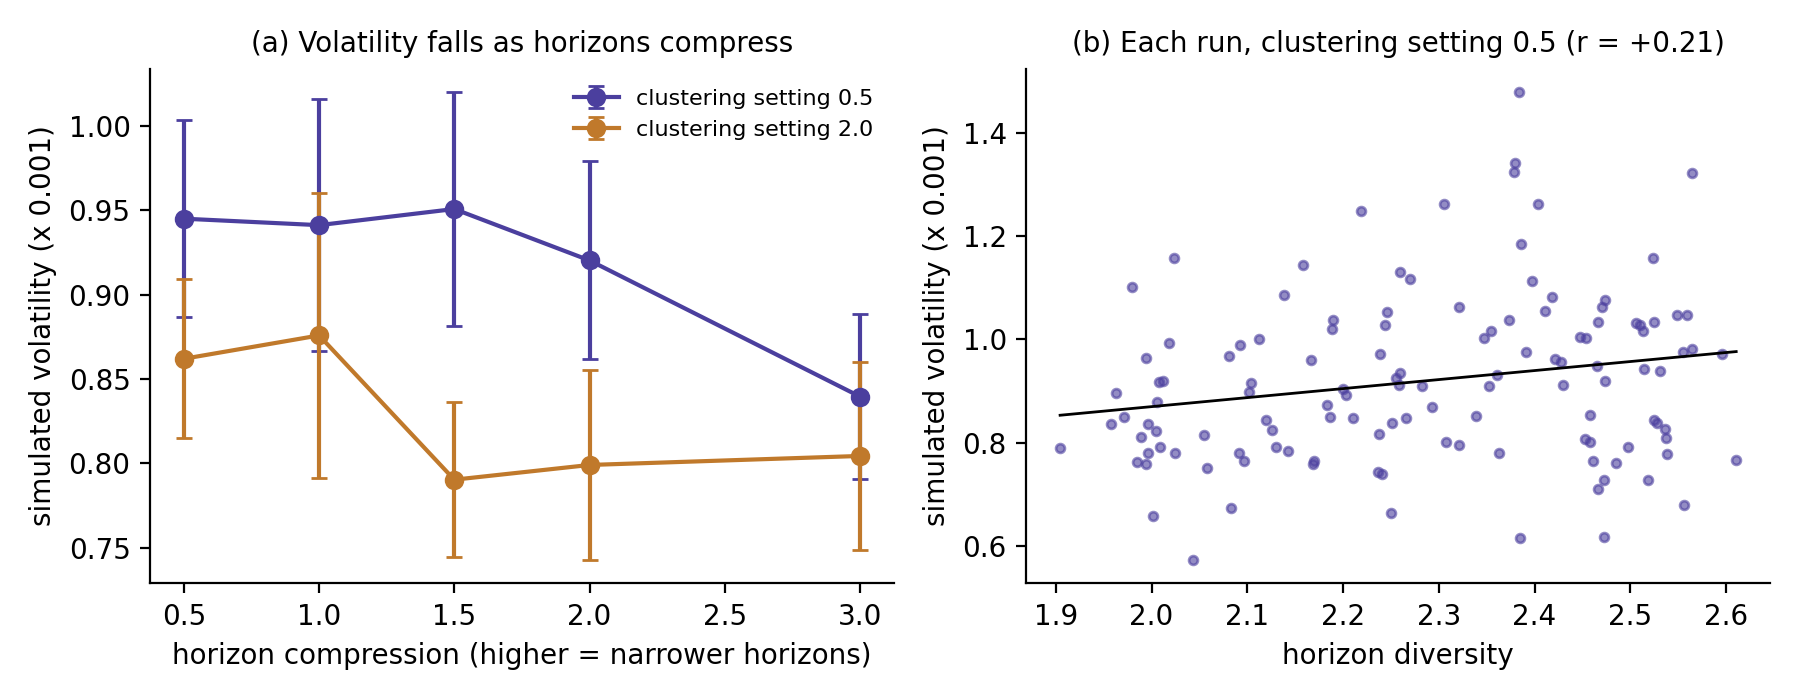
\includegraphics[width=0.95\linewidth]{conc_check}
\caption{(a) Simulated volatility against horizon compression for two clustering strengths (error bars are 95\% ranges for the mean). (b) Each simulation run at clustering strength 0.5: more diverse horizons go with slightly higher volatility.}
\label{fig:conc}
\end{figure}

\subsection{Why the model behaves this way}

The explanation is the friction channel of Eq.~\eqref{eq:sigeff}. When investors' horizons are close together, the average distance between an investor and their counterparties is small, so noise is low and volatility is lower. More diverse horizons mean more cross-horizon friction and more noise. The model contains \emph{no} mechanism by which concentrated horizons make the market \emph{fragile}: nothing weakens when diversity is lost, so nothing amplifies a shock. The fragility channel that the Fractal Market Hypothesis describes remains a verbal idea in our model, not something the simulation generates.

\begin{keyidea}[The tension in one sentence]
In the model, less diverse horizons \emph{reduce} volatility through lower friction; in the stock data, owners with similar horizons go with \emph{higher} volatility, a small effect in the direction the Fractal Market Hypothesis predicts but the opposite direction to the model's own simulated channel.
\end{keyidea}

We have corrected the paper to say this. We also note that the data effect is small and comes from a survivors-only sample, so it may not be reliable. The disagreement is real, but it does not by itself tell us which side is wrong.

\subsection{Options for the model}

If the aim is a model whose simulated behaviour agrees with the data, the model needs a channel through which the loss of horizon diversity makes the market fragile. We see three options.

\begin{description}[leftmargin=1.2em,style=nextline]
\item[Option A: a horizon-dependent stabiliser.] Make the value-investing force (the term with weight $\bar\alpha$ in Eq.~\eqref{eq:demand}) weaker when horizons are concentrated, representing the fact that long-horizon value investors are the ones who step in during a sell-off. \emph{For:} it directly produces the fragility the hypothesis describes, so model and data could agree. \emph{Against:} it requires re-verifying every simulation result, and because it is introduced after seeing the data it risks looking like building the answer we wanted. It must be reported openly as a post-hoc change.
\item[Option B: horizon-dependent liquidity.] Add a liquidity-provider role whose willingness to absorb trades depends on how many counterparties with different horizons are available, so that concentrated horizons reduce market depth and raise the price impact $\lambda$. \emph{For:} closer to the disagreement-and-volume mechanism of \citet{harrisraviv1993} and to the real way horizons are supposed to matter. \emph{Against:} a larger redesign with new parameters.
\item[Option C: keep the model and report the tension.] Describe the model as capturing only the friction channel, say plainly that the data point to a channel it does not contain, and treat that as an open question. \emph{For:} simple and honest. \emph{Against:} a weaker contribution, since the model then does not explain the stock-level evidence.
\end{description}

We have not chosen among these. We think the choice depends partly on how a referee would view post-hoc model changes, which is a question for experienced researchers in the field, and we are seeking advice on it.

\section{Corrections Made Along the Way}
\label{sec:corrections}

Several earlier claims did not survive closer examination. We list them together so that a reader can see exactly what changed. Each was corrected in the paper.

\begin{table}[htbp]
\centering
\caption{Earlier claims, what we found, and what the text now says.}
\label{tab:corr}
\small
\begin{tabular}{p{0.07\linewidth}p{0.27\linewidth}p{0.30\linewidth}p{0.28\linewidth}}
\toprule
 & \textbf{Earlier claim} & \textbf{What we found} & \textbf{Now}\\
\midrule
1 & Corrected statistic for the clustering score is about 15, with an effective sample of 17 (``17 lags'') & Never computed. Real Newey--West: $t=19.0$ at 3 lags, $16.3$ at 8; effective sample about 24 & Reported with a lag table and lag-choice rules\\
2 & Clustering significant at $p<0.001$ in every quarter & The pairwise test overstates significance. Permutation test: 48 of 50 quarters at 5\%, 47 of 50 at 1\% & Reported as 48 of 50\\
3 & Horizon diversity versus VIX ($r=-0.53$) validates the model & Largely price drift. Share-based turnover gives $r=-0.06$ & Reframed as a measurement artifact\\
4 & Granger result ``confirms'' the model's channel & Direction is the reverse of the model, and does not reproduce on a rebuilt series & Marked suggestive\\
5 & Temporal liquidity versus VIX validates the model; sample of 36 quarters & Sample is 45 quarters; correlation is mostly mechanical because volatility is inside TL; autocorrelation part unrelated to VIX ($+0.04$) & Reported as mechanical\\
6 & The MOVE index was ours & It is a published ICE Bank of America index & Described correctly\\
7 & Compressing horizons raises simulated volatility & The sweep never fed the compressed horizons into the simulation. Properly done, volatility falls & Replaced with the real result\\
8 & The uniform price mode bounded by $0.0016$ with no derivation & Derived gain is $\lambda n\bar\beta/\bar p\approx 0.0013$ & Derivation added\\
9 & Temporal liquidity peaks at moderate clustering & Very large run-to-run spread; peak not statistically reliable & Treated with caution\\
10 & Related work & Closest empirical overlap (Cella et al., 2013) was not cited & Cited and differences stated\\
\bottomrule
\end{tabular}
\end{table}

\section{Limitations and Threats to Validity}
\label{sec:limits}

We collect here the main reasons the results should be read with care.

\begin{enumerate}[leftmargin=*]
\item \textbf{Horizons are inferred, not observed.} The mapping $\tau=63/\theta$ from turnover to a horizon is a rough device. It cannot see trading within a quarter, short positions or derivatives, and the sample is tilted toward slow institutions.
\item \textbf{The share-based turnover result rests on our own rebuild.} The rebuilt diversity series correlates only $0.50$ with the original, with a particularly large gap in 2022 Q4. We have not identified the source. An independent check by someone else on the team is warranted before the conclusion is relied upon.
\item \textbf{The stock-level sample is survivors only.} Free price data omit delisted and acquired companies, and only about 60\% of securities could be matched to tickers.
\item \textbf{The stock-level effect is small.} Within a stock, one standard deviation of owner spread moves next-quarter volatility by about 1\% of a standard deviation, and only with share-based horizons.
\item \textbf{The panel is limited.} The holdings cover 150 managers. The clustering score and the owner-spread measure are computed from those managers only.
\item \textbf{Holdings are not trades.} The clustering score measures similarity of holdings, not of purchases.
\item \textbf{The model and the stock-level result disagree in sign} (Section~\ref{sec:tension}). Whether this is a flaw in the model, in the data, or in how the hypothesis maps onto the model is open.
\item \textbf{The model is stylised.} Horizons are exogenous, trading goes through a single market maker, the fundamental value is a simple random walk, and the market has only 80 investors. Results at 160 and 320 investors point the same way, but this is not a model of any specific market.
\item \textbf{Bond results are descriptive.} Seven funds, 27 quarters each, one fund family.
\item \textbf{Some earlier numbers rest on approximations or single runs.} For example, the belief-fragmentation ratio has large run-to-run variation.
\end{enumerate}

\section{Future Work}
\label{sec:future}

\subsection{Access to the standard stock database}

The most valuable data upgrade is CRSP, the Center for Research in Security Prices, a standard database in finance that holds every US stock back to 1926 including those later delisted, with market capitalisation, trading volume and carefully adjusted returns. Universities usually provide access through Wharton Research Data Services (WRDS). WRDS also provides the full 13F holdings database covering all managers, not just our 150. With it we could:
\begin{itemize}[leftmargin=*]
\item repeat the stock-level test on the full universe, removing the survivorship bias and the ticker-matching loss;
\item control for firm size and trading volume properly;
\item test more outcomes, such as crash risk, co-movement with the market, and liquidity measures; and
\item use all managers when measuring owner horizons.
\end{itemize}
This is the single step most likely to settle whether the small stock-level effect is real. We are seeking access.

\subsection{Other next steps}
\begin{itemize}[leftmargin=*]
\item \textbf{Rebuild the aggregate diversity measure from share-based turnover throughout}, and resolve the discrepancy with the original series.
\item \textbf{Decide on the model change} described in Section~\ref{sec:tension}, and if one is made, re-verify every simulation result.
\item \textbf{Use trade-level data} to separate the behavioural link between volatility and trading speed from price drift, and to test whether like-horizon investors \emph{buy} the same securities.
\item \textbf{Improve the bond test} with insurer bond filings (NAIC Schedule D), which record actual portfolio turnover, and with a larger set of bond funds across families.
\item \textbf{Derive horizons from limited attention} \citep{sims2003} so that they are an outcome of the model, not an input.
\item \textbf{Add an information-asymmetry channel} in the spirit of \citet{kyle1985} and \citet{akerlof1970}, in which a long-horizon investor discounts prices proposed by short-horizon investors who may know more.
\end{itemize}

\section{Conclusion}
\label{sec:conclusion}

We set out to ask whether the diversity of investor time horizons matters for market stability, and to make the Fractal Market Hypothesis concrete. We built a model in which investors with similar horizons cluster and drift together. In the model, clustering lowers volatility and nearly eliminates belief fragmentation, while drift steadily erodes horizon diversity.

The real-data results are more mixed than we first believed. The model's central assumption holds: investors with similar horizons really do hold more similar portfolios, an effect that is modest but consistent and robust to careful statistical correction. Our first headline empirical result, a link between horizon diversity and the VIX, does not survive when price movements are removed from the turnover measure, and we report it as a measurement artifact. At the level of individual stocks, similar-horizon owners go with slightly higher volatility, as the hypothesis predicts, though the effect is small and opposite in sign to what our own model simulates.

We think the most useful outcome of this work is an honest map of what is and is not established: a clean test of the model's key assumption, a demonstration of a measurement trap that affects any study inferring horizons from holdings, and a clearly identified gap between the model's simulated channel and the fragility the hypothesis is about. Closing that gap, with better data and a revised model, is the next step.

\appendix

\section{Glossary of Terms}
\label{app:glossary}

\begin{longtable}{p{0.27\linewidth}p{0.66\linewidth}}
\toprule
\textbf{Term} & \textbf{Plain-English meaning}\\
\midrule
\endhead
Trading horizon ($\tau$) & How long an investor typically holds a position and looks back at prices, in trading days.\\
Chronotype & Our word for an investor's natural trading horizon.\\
Horizon clustering ($\kappa_h$, ``temporal homophily'') & The tendency for investors with similar horizons to deal with each other. In the model, a dial; in the data, estimated as a correlation.\\
Horizon clustering score ($\hat\kappa_h$) & The estimated clustering in real data: the correlation, across pairs of managers, between how close their horizons are and how similar their portfolios are.\\
Horizon diversity (TDI) & How spread out investors' horizons are, measured by the entropy of the share of investors in 16 log-scale bins. Zero if all in one bin.\\
Belief fragmentation (TMFI) & How much average beliefs about the price differ between horizon groups.\\
Temporal liquidity (TL) & One divided by the product of return volatility and the size of the first autocorrelation. Higher means smoother price discovery.\\
Fractal Market Hypothesis & The idea that markets are stable when investors have many different time horizons and fragile when horizons converge.\\
Turnover & The share of a portfolio that changed from one quarter to the next.\\
Price drift & Change in portfolio weights caused by price movements rather than trading.\\
Form 13F & Quarterly report of stock holdings filed with the SEC by large investment managers.\\
Form N-PORT & The analogous holdings report for registered funds, including bond funds.\\
CUSIP & A nine-character code that uniquely identifies a security.\\
VIX & Published index of expected US stock-market volatility (``fear gauge'').\\
MOVE & Published ICE Bank of America index of expected Treasury-bond volatility.\\
Weighted average maturity & The dollar-weighted average years remaining to maturity of a bond fund's holdings.\\
Cosine similarity & A number from 0 to 1 measuring how alike two lists of weights are.\\
Correlation & A number from $-1$ to $+1$ measuring how closely two series move together.\\
$t$-statistic, $p$-value & Measures of how surprising a result would be by luck alone. A $t$ above about 2, or a $p$ below 0.05, is conventionally significant.\\
Newey--West correction & An adjustment to uncertainty estimates for data in which each observation resembles its neighbours. It needs a number of \emph{lags}.\\
Block bootstrap & Resampling blocks of consecutive observations to estimate uncertainty without assuming independence.\\
Permutation test & Shuffling a variable many times to see how often chance alone produces a result as strong as the real one.\\
Granger test & Asks whether past values of one series help predict another beyond that series' own past. A test of lead and lag, not proof of cause.\\
Fama--MacBeth regression & Run a regression separately each period, then average the coefficients over time.\\
Fixed effects & Controls that remove anything constant about a stock (or about a period), so that comparisons are within a stock (or period).\\
Placebo test & A test using shuffled or irrelevant data that should show no effect; it checks that the method does not manufacture results.\\
Survivorship bias & Distortion from only including companies that still exist.\\
CRSP, WRDS & The standard university database of US stock prices (CRSP) and the service that provides access to it (Wharton Research Data Services).\\
Fiedler value ($\lambda_2$) & A standard measure of how well connected a network is.\\
Assortativity & Correlation between a node's characteristic and its neighbours' characteristics. High means like links with like.\\
\bottomrule
\end{longtable}

\section{Model Parameters}
\label{app:params}

\begin{table}[htbp]
\centering
\begin{tabular}{llr}
\toprule
Parameter & Meaning & Value\\
\midrule
$n$ & Number of simulated investors & 80\\
$T$ & Periods per run (after a 500-period burn-in) & 500\\
$\lambda$ & Price impact of net demand & 0.008\\
$\bar\alpha$ & Value-investing weight & 0.30\\
$\bar\beta$ & Trend-following weight & 0.20\\
$\sigma_F$ & Volatility of the fundamental value & 0.010\\
$\sigma_0$ & Base demand noise & 1.0\\
$\gamma$ & Cross-horizon friction coefficient & 0.20\\
$\sigma_{\mathrm{obs}}$ & Observation noise for belief fragmentation & 0.008\\
$\eta$ & Horizon adaptation rate & 0.06\\
$\kappa_h$ & Horizon clustering strength (swept) & 0 to 6\\
Seeds & Random-number seeds per setting & 30 (10 for asset-class sweep)\\
\bottomrule
\end{tabular}
\end{table}

\section{Data Handling Rules}
\label{app:checks}

\begin{itemize}[leftmargin=*]
\item Holdings: only positions with strictly positive value are kept (and positive share counts when shares are used), so no logarithm of zero or division by zero arises.
\item Managers with quarterly turnover below 0.1\% are dropped.
\item Horizons are limited to 5 to 2{,}000 trading days.
\item Horizon diversity: quarters need at least 50 reporting managers (45 quarters qualify, 2013 Q3 to 2024 Q3).
\item Clustering score: quarters need at least 8 managers with valid horizons and at least 20 pairs (50 quarters qualify).
\item Share-based turnover: a single price per security (the implied price from reported value and shares) for both quarters; positions whose share count changes by almost exactly a split ratio (2, 3, 4, 5, 6, 8, 10 or 20, or their inverses) are rebased before measuring trades.
\item Bond funds: par amount and market value used; bonds that matured between reports are not counted as trades; only consecutive reports 60 to 125 days apart are used.
\item Stock-level test: at least 10 owners per stock, at least 50 trading days of prices in a quarter, quarters with fewer than 60 stocks skipped in the quarter-by-quarter regressions.
\item Quarterly VIX and MOVE: averages of the published values within each quarter.
\end{itemize}

\section{Additional Results}
\label{app:extra}

\begin{table}[htbp]
\centering
\caption{All stock-level results (standardised coefficients on owner-horizon spread). Newey--West errors for the quarter-by-quarter method; stock-clustered errors for the others.}
\small
\begin{tabular}{llrr}
\toprule
Outcome & Method & Share-based & Weight-based\\
\midrule
Next-quarter volatility (log) & Quarter-by-quarter average & $-0.0459$ ($t=-6.20$) & $-0.0440$ ($t=-8.04$)\\
 & Pooled, quarter effects & $-0.0169$ ($t=-4.13$) & $-0.0089$ ($t=-2.33$)\\
 & Stock and quarter effects & $-0.0106$ ($t=-2.42$) & $-0.0047$ ($t=-1.13$)\\
Worst daily return next quarter & Quarter-by-quarter average & $+0.0417$ ($t=4.47$) & $+0.0416$ ($t=4.73$)\\
 & Pooled, quarter effects & $-0.0038$ ($t=-0.58$) & $-0.0064$ ($t=-1.07$)\\
Skewness next quarter & Quarter-by-quarter average & $-0.0006$ ($t=-0.09$) & $+0.0025$ ($t=+0.38$)\\
 & Pooled, quarter effects & $-0.0053$ ($t=-0.68$) & $+0.0009$ ($t=+0.13$)\\
Placebo (volatility) & Quarter-by-quarter average & $0.0000$ ($t=0.01$) & not run\\
\bottomrule
\end{tabular}
\end{table}

\begin{table}[htbp]
\centering
\caption{Autocorrelation of the quarterly clustering score at lags 1 to 8 and Ljung--Box tests.}
\small
\begin{tabular}{lrrrrrrrr}
\toprule
Lag & 1 & 2 & 3 & 4 & 5 & 6 & 7 & 8\\
\midrule
Autocorrelation & 0.346 & 0.247 & 0.146 & 0.093 & 0.051 & 0.164 & 0.058 & 0.028\\
\bottomrule
\end{tabular}

\vspace{4pt}
Ljung--Box $p$-values: 0.012 (1 lag), 0.008 (2 lags), 0.023 (4 lags), 0.102 (8 lags).
\end{table}

\section{Reproducing the Results}
\label{app:repro}

All code is in the project folder \texttt{cme\_validation}. The main files are listed below in the order they are run.

\begin{center}
\small
\begin{tabular}{p{0.38\linewidth}p{0.52\linewidth}}
\toprule
File & Purpose\\
\midrule
\texttt{cme\_canonical.py} & The simulation model and all simulation results.\\
\texttt{verify\_numbers.py} & 30-seed paired replication of the volatility and fragmentation ratios.\\
\texttt{empirical\_tdi.py} & Downloads holdings and builds the original horizon diversity series.\\
\texttt{kappa\_empirical.py} & Computes the clustering score each quarter.\\
\texttt{kappa\_hac\_tests.py} & Newey--West at several lags, bootstrap and permutation test.\\
\texttt{price\_adjusted\_tdi.py} & Share-based turnover and the price-drift comparison.\\
\texttt{bond\_empirical.py}, \texttt{bond\_by\_type.py} & Bond fund analyses.\\
\texttt{map\_cusips.py}, \texttt{stock\_prices.py} & Security-to-ticker mapping and price download.\\
\texttt{stock\_level\_test.py} & The stock-level test.\\
\texttt{sim\_concentration\_check.py} & Horizon-compression experiment in the simulation.\\
\texttt{worked\_example.py} & Prints the three-manager worked example.\\
\bottomrule
\end{tabular}
\end{center}


\bibliographystyle{plainnat}
\renewcommand{\refname}{References}\begin{thebibliography}{25}

\bibitem[Amihud and Mendelson(1986)]{amihud1986}
Amihud, Y., Mendelson, H., 1986.
Asset pricing and the bid-ask spread.
\textit{Journal of Financial Economics} 17 (2), 223--249.

\bibitem[Acemoglu et al.(2015)]{acemoglu2015}
Acemoglu, D., Ozdaglar, A., Tahbaz-Salehi, A., 2015.
Systemic risk and stability in financial networks.
\textit{American Economic Review} 105 (2), 564--608.

\bibitem[Arthur et al.(1997)]{arthur1997}
Arthur, W.B., Holland, J.H., LeBaron, B., Palmer, R., Tayler, P., 1997.
Asset pricing under endogenous expectations in an artificial stock market.
In: Arthur, W.B., Durlauf, S.N., Lane, D.A. (Eds.),
\textit{The Economy as an Evolving Complex System~II}.
Addison-Wesley, pp.\ 15--44.

\bibitem[Bikhchandani et al.(1992)]{bikhchandani1992}
Bikhchandani, S., Hirshleifer, D., Welch, I., 1992.
A theory of fads, fashion, custom, and cultural change as informational
cascades.
\textit{Journal of Political Economy} 100 (5), 992--1026.

\bibitem[Del~Guercio and Tkac(2002)]{delguercio2002}
Del~Guercio, D., Tkac, P.A., 2002.
The determinants of the flow of funds of managed portfolios:
Mutual funds versus pension funds.
\textit{Journal of Financial and Quantitative Analysis} 37 (4), 523--557.

\bibitem[Caplin and Dean(2015)]{caplin2015}
Caplin, A., Dean, M., 2015.
Revealed preference, rational inattention, and costly information acquisition.
\textit{American Economic Review} 105 (7), 2183--2203.

\bibitem[Cont(2001)]{cont2001}
Cont, R., 2001.
Empirical properties of asset returns: stylized facts and statistical issues.
\textit{Quantitative Finance} 1 (2), 223--236.

\bibitem[Corsi(2009)]{corsi2009}
Corsi, F., 2009.
A simple approximate long-memory model of realized volatility.
\textit{Journal of Financial Econometrics} 7 (2), 174--196.

\bibitem[Devenow and Welch(1996)]{devenow1996}
Devenow, A., Welch, I., 1996.
Rational herding in financial economics.
\textit{European Economic Review} 40 (3--5), 603--615.

\bibitem[French and Roll(1986)]{frenchroll1986}
French, K.R., Roll, R., 1986.
Stock return variances: The arrival of information and the reaction
of traders.
\textit{Journal of Financial Economics} 17 (1), 5--26.

\bibitem[Farmer and Foley(2009)]{farmerfoley2009}
Farmer, J.D., Foley, D., 2009.
The economy needs agent-based modelling.
\textit{Nature} 460 (7256), 685--686.

\bibitem[Golub and Jackson(2012)]{golub2012}
Golub, B., Jackson, M.O., 2012.
How homophily affects the speed of learning and best-response dynamics.
\textit{Quarterly Journal of Economics} 127 (3), 1287--1338.

\bibitem[LeBaron(2001)]{lebaron2001}
LeBaron, B., 2001.
A builder's guide to agent-based financial markets.
\textit{Quantitative Finance} 1 (2), 254--261.

\bibitem[M{\"u}ller et al.(1993)]{muller1993}
M{\"u}ller, U.A., Dacorogna, M.M., Dav{\'e}, R.D., Olsen, R.B.,
Pictet, O.V., von Weizs{\"a}cker, J.E., 1993.
Fractals and intrinsic time---a challenge to investment managers.
Working Paper, Olsen \& Associates, Zurich.
Available at: \url{https://ssrn.com/abstract=5302}.

\bibitem[Peters(1994)]{peters1994}
Peters, E.E., 1994.
\textit{Fractal Market Analysis: Applying Chaos Theory to Investment and
Economics}.
Wiley Finance Editions, New York.

\bibitem[Sims(2003)]{sims2003}
Sims, C.A., 2003.
Implications of rational inattention.
\textit{Journal of Monetary Economics} 50 (3), 665--690.

\bibitem[Akerlof(1970)]{akerlof1970}
Akerlof, G.A., 1970.
The market for ``lemons'': Quality uncertainty and the market mechanism.
\textit{Quarterly Journal of Economics} 84 (3), 488--500.

\bibitem[Kyle(1985)]{kyle1985}
Kyle, A.S., 1985.
Continuous auctions and insider trading.
\textit{Econometrica} 53 (6), 1315--1335.

\bibitem[Baker et al.(2016)]{baker2016}
Baker, S.R., Bloom, N., Davis, S.J., 2016.
Measuring economic policy uncertainty.
\textit{Quarterly Journal of Economics} 131 (4), 1593--1636.

\bibitem[Bushee(1998)]{bushee1998}
Bushee, B.J., 1998.
The influence of institutional investors on myopic R\&D investment behavior.
\textit{The Accounting Review} 73 (3), 305--333.

\bibitem[Cella et al.(2013)]{cella2013}
Cella, C., Ellul, A., Giannetti, M., 2013.
Investors' horizons and the amplification of market shocks.
\textit{Review of Financial Studies} 26 (7), 1607--1648.

\bibitem[Gaspar et al.(2005)]{gaspar2005}
Gaspar, J.-M., Massa, M., Matos, P., 2005.
Shareholder investment horizons and the market for corporate control.
\textit{Journal of Financial Economics} 76 (1), 135--165.

\bibitem[Kristoufek(2012)]{kristoufek2012}
Kristoufek, L., 2012.
Fractal markets hypothesis and the global financial crisis: scaling,
investment horizons and liquidity.
\textit{Advances in Complex Systems} 15 (6), 1250065.

\bibitem[Li et al.(2014)]{li2014}
Li, D.-Y., Nishimura, Y., Men, M., 2014.
Fractal markets: liquidity and investors on different time horizons.
\textit{Physica A} 407, 144--151.

\bibitem[Harris and Raviv(1993)]{harrisraviv1993}
Harris, M., Raviv, A., 1993.
Differences of opinion make a horse race.
\textit{Review of Financial Studies} 6 (3), 473--506.

\end{thebibliography}

\end{document}
